% Options for packages loaded elsewhere
\PassOptionsToPackage{unicode}{hyperref}
\PassOptionsToPackage{hyphens}{url}
\PassOptionsToPackage{dvipsnames,svgnames,x11names}{xcolor}
%
\documentclass[
  letterpaper,
  DIV=11,
  numbers=noendperiod,
  oneside]{scrreprt}

\usepackage{amsmath,amssymb}
\usepackage{lmodern}
\usepackage{iftex}
\ifPDFTeX
  \usepackage[T1]{fontenc}
  \usepackage[utf8]{inputenc}
  \usepackage{textcomp} % provide euro and other symbols
\else % if luatex or xetex
  \usepackage{unicode-math}
  \defaultfontfeatures{Scale=MatchLowercase}
  \defaultfontfeatures[\rmfamily]{Ligatures=TeX,Scale=1}
\fi
% Use upquote if available, for straight quotes in verbatim environments
\IfFileExists{upquote.sty}{\usepackage{upquote}}{}
\IfFileExists{microtype.sty}{% use microtype if available
  \usepackage[]{microtype}
  \UseMicrotypeSet[protrusion]{basicmath} % disable protrusion for tt fonts
}{}
\makeatletter
\@ifundefined{KOMAClassName}{% if non-KOMA class
  \IfFileExists{parskip.sty}{%
    \usepackage{parskip}
  }{% else
    \setlength{\parindent}{0pt}
    \setlength{\parskip}{6pt plus 2pt minus 1pt}}
}{% if KOMA class
  \KOMAoptions{parskip=half}}
\makeatother
\usepackage{xcolor}
\usepackage[left=1in,marginparwidth=2.0666666666667in,textwidth=4.1333333333333in,marginparsep=0.3in]{geometry}
\setlength{\emergencystretch}{3em} % prevent overfull lines
\setcounter{secnumdepth}{5}
% Make \paragraph and \subparagraph free-standing
\ifx\paragraph\undefined\else
  \let\oldparagraph\paragraph
  \renewcommand{\paragraph}[1]{\oldparagraph{#1}\mbox{}}
\fi
\ifx\subparagraph\undefined\else
  \let\oldsubparagraph\subparagraph
  \renewcommand{\subparagraph}[1]{\oldsubparagraph{#1}\mbox{}}
\fi

\usepackage{color}
\usepackage{fancyvrb}
\newcommand{\VerbBar}{|}
\newcommand{\VERB}{\Verb[commandchars=\\\{\}]}
\DefineVerbatimEnvironment{Highlighting}{Verbatim}{commandchars=\\\{\}}
% Add ',fontsize=\small' for more characters per line
\newenvironment{Shaded}{}{}
\newcommand{\AlertTok}[1]{\textcolor[rgb]{1.00,0.33,0.33}{\textbf{#1}}}
\newcommand{\AnnotationTok}[1]{\textcolor[rgb]{0.42,0.45,0.49}{#1}}
\newcommand{\AttributeTok}[1]{\textcolor[rgb]{0.84,0.23,0.29}{#1}}
\newcommand{\BaseNTok}[1]{\textcolor[rgb]{0.00,0.36,0.77}{#1}}
\newcommand{\BuiltInTok}[1]{\textcolor[rgb]{0.84,0.23,0.29}{#1}}
\newcommand{\CharTok}[1]{\textcolor[rgb]{0.01,0.18,0.38}{#1}}
\newcommand{\CommentTok}[1]{\textcolor[rgb]{0.42,0.45,0.49}{#1}}
\newcommand{\CommentVarTok}[1]{\textcolor[rgb]{0.42,0.45,0.49}{#1}}
\newcommand{\ConstantTok}[1]{\textcolor[rgb]{0.00,0.36,0.77}{#1}}
\newcommand{\ControlFlowTok}[1]{\textcolor[rgb]{0.84,0.23,0.29}{#1}}
\newcommand{\DataTypeTok}[1]{\textcolor[rgb]{0.84,0.23,0.29}{#1}}
\newcommand{\DecValTok}[1]{\textcolor[rgb]{0.00,0.36,0.77}{#1}}
\newcommand{\DocumentationTok}[1]{\textcolor[rgb]{0.42,0.45,0.49}{#1}}
\newcommand{\ErrorTok}[1]{\textcolor[rgb]{1.00,0.33,0.33}{\underline{#1}}}
\newcommand{\ExtensionTok}[1]{\textcolor[rgb]{0.84,0.23,0.29}{\textbf{#1}}}
\newcommand{\FloatTok}[1]{\textcolor[rgb]{0.00,0.36,0.77}{#1}}
\newcommand{\FunctionTok}[1]{\textcolor[rgb]{0.44,0.26,0.76}{#1}}
\newcommand{\ImportTok}[1]{\textcolor[rgb]{0.01,0.18,0.38}{#1}}
\newcommand{\InformationTok}[1]{\textcolor[rgb]{0.42,0.45,0.49}{#1}}
\newcommand{\KeywordTok}[1]{\textcolor[rgb]{0.84,0.23,0.29}{#1}}
\newcommand{\NormalTok}[1]{\textcolor[rgb]{0.14,0.16,0.18}{#1}}
\newcommand{\OperatorTok}[1]{\textcolor[rgb]{0.14,0.16,0.18}{#1}}
\newcommand{\OtherTok}[1]{\textcolor[rgb]{0.44,0.26,0.76}{#1}}
\newcommand{\PreprocessorTok}[1]{\textcolor[rgb]{0.84,0.23,0.29}{#1}}
\newcommand{\RegionMarkerTok}[1]{\textcolor[rgb]{0.42,0.45,0.49}{#1}}
\newcommand{\SpecialCharTok}[1]{\textcolor[rgb]{0.00,0.36,0.77}{#1}}
\newcommand{\SpecialStringTok}[1]{\textcolor[rgb]{0.01,0.18,0.38}{#1}}
\newcommand{\StringTok}[1]{\textcolor[rgb]{0.01,0.18,0.38}{#1}}
\newcommand{\VariableTok}[1]{\textcolor[rgb]{0.89,0.38,0.04}{#1}}
\newcommand{\VerbatimStringTok}[1]{\textcolor[rgb]{0.01,0.18,0.38}{#1}}
\newcommand{\WarningTok}[1]{\textcolor[rgb]{1.00,0.33,0.33}{#1}}

\providecommand{\tightlist}{%
  \setlength{\itemsep}{0pt}\setlength{\parskip}{0pt}}\usepackage{longtable,booktabs,array}
\usepackage{calc} % for calculating minipage widths
% Correct order of tables after \paragraph or \subparagraph
\usepackage{etoolbox}
\makeatletter
\patchcmd\longtable{\par}{\if@noskipsec\mbox{}\fi\par}{}{}
\makeatother
% Allow footnotes in longtable head/foot
\IfFileExists{footnotehyper.sty}{\usepackage{footnotehyper}}{\usepackage{footnote}}
\makesavenoteenv{longtable}
\usepackage{graphicx}
\makeatletter
\def\maxwidth{\ifdim\Gin@nat@width>\linewidth\linewidth\else\Gin@nat@width\fi}
\def\maxheight{\ifdim\Gin@nat@height>\textheight\textheight\else\Gin@nat@height\fi}
\makeatother
% Scale images if necessary, so that they will not overflow the page
% margins by default, and it is still possible to overwrite the defaults
% using explicit options in \includegraphics[width, height, ...]{}
\setkeys{Gin}{width=\maxwidth,height=\maxheight,keepaspectratio}
% Set default figure placement to htbp
\makeatletter
\def\fps@figure{htbp}
\makeatother

\KOMAoption{captions}{tableheading}
\makeatletter
\@ifpackageloaded{tcolorbox}{}{\usepackage[many]{tcolorbox}}
\@ifpackageloaded{fontawesome5}{}{\usepackage{fontawesome5}}
\definecolor{quarto-callout-color}{HTML}{909090}
\definecolor{quarto-callout-note-color}{HTML}{0758E5}
\definecolor{quarto-callout-important-color}{HTML}{CC1914}
\definecolor{quarto-callout-warning-color}{HTML}{EB9113}
\definecolor{quarto-callout-tip-color}{HTML}{00A047}
\definecolor{quarto-callout-caution-color}{HTML}{FC5300}
\definecolor{quarto-callout-color-frame}{HTML}{acacac}
\definecolor{quarto-callout-note-color-frame}{HTML}{4582ec}
\definecolor{quarto-callout-important-color-frame}{HTML}{d9534f}
\definecolor{quarto-callout-warning-color-frame}{HTML}{f0ad4e}
\definecolor{quarto-callout-tip-color-frame}{HTML}{02b875}
\definecolor{quarto-callout-caution-color-frame}{HTML}{fd7e14}
\makeatother
\makeatletter
\makeatother
\makeatletter
\@ifpackageloaded{bookmark}{}{\usepackage{bookmark}}
\makeatother
\makeatletter
\@ifpackageloaded{caption}{}{\usepackage{caption}}
\AtBeginDocument{%
\ifdefined\contentsname
  \renewcommand*\contentsname{Table of contents}
\else
  \newcommand\contentsname{Table of contents}
\fi
\ifdefined\listfigurename
  \renewcommand*\listfigurename{List of Figures}
\else
  \newcommand\listfigurename{List of Figures}
\fi
\ifdefined\listtablename
  \renewcommand*\listtablename{List of Tables}
\else
  \newcommand\listtablename{List of Tables}
\fi
\ifdefined\figurename
  \renewcommand*\figurename{Figure}
\else
  \newcommand\figurename{Figure}
\fi
\ifdefined\tablename
  \renewcommand*\tablename{Table}
\else
  \newcommand\tablename{Table}
\fi
}
\@ifpackageloaded{float}{}{\usepackage{float}}
\floatstyle{ruled}
\@ifundefined{c@chapter}{\newfloat{codelisting}{h}{lop}}{\newfloat{codelisting}{h}{lop}[chapter]}
\floatname{codelisting}{Listing}
\newcommand*\listoflistings{\listof{codelisting}{List of Listings}}
\makeatother
\makeatletter
\@ifpackageloaded{caption}{}{\usepackage{caption}}
\@ifpackageloaded{subcaption}{}{\usepackage{subcaption}}
\makeatother
\makeatletter
\@ifpackageloaded{tcolorbox}{}{\usepackage[many]{tcolorbox}}
\makeatother
\makeatletter
\@ifundefined{shadecolor}{\definecolor{shadecolor}{rgb}{.97, .97, .97}}
\makeatother
\makeatletter
\@ifpackageloaded{sidenotes}{}{\usepackage{sidenotes}}
\@ifpackageloaded{marginnote}{}{\usepackage{marginnote}}
\makeatother
\makeatletter
\makeatother
\ifLuaTeX
  \usepackage{selnolig}  % disable illegal ligatures
\fi
\IfFileExists{bookmark.sty}{\usepackage{bookmark}}{\usepackage{hyperref}}
\IfFileExists{xurl.sty}{\usepackage{xurl}}{} % add URL line breaks if available
\urlstyle{same} % disable monospaced font for URLs
\hypersetup{
  pdftitle={Open Manual for Dr.~Hu's Amazing Team},
  pdfauthor={胡悦},
  colorlinks=true,
  linkcolor={blue},
  filecolor={Maroon},
  citecolor={Blue},
  urlcolor={Blue},
  pdfcreator={LaTeX via pandoc}}

\title{Open Manual for Dr.~Hu's Amazing Team}
\author{胡悦}
\date{2022-10-11T00:00:00+08:00}

\begin{document}
\maketitle
\ifdefined\Shaded\renewenvironment{Shaded}{\begin{tcolorbox}[frame hidden, borderline west={3pt}{0pt}{shadecolor}, enhanced, interior hidden, boxrule=0pt, breakable, sharp corners]}{\end{tcolorbox}}\fi

\renewcommand*\contentsname{Table of contents}
{
\hypersetup{linkcolor=}
\setcounter{tocdepth}{2}
\tableofcontents
}
\bookmarksetup{startatroot}

\hypertarget{ux524dux8a00}{%
\chapter*{前言}\label{ux524dux8a00}}
\addcontentsline{toc}{chapter}{前言}

亲爱的朋友:

如果你正打算阅读这本\emph{Open Manual for Dr.~Hu's Amazing
Team},那说明你正逢和一个非常棒的团队合作的机会。
我们队伍中的成员来自五湖四海,但都对基于政治认知解密政治态度、政治身份、政治传播和社会经济不平等的议题抱有兴趣。
大家秉承``\textbf{立场坚定、个性自由}''的共识和严守科学规范的操守,为有趣的题目、为自身的发展(当然,也为情怀)而进行政治科学研究。
既能百花齐放,也有同心协力。

为了组内成员能够有效交流,高效合作,我编纂了这本小册子。
希望新加入的你能通过阅读和学习,在操作层面更好融入我们的工作流程,实现顺畅合作,最终达成你和团队的共同成长。
有一点有必要说明,这本小册子的目的不在于``一本在手,天下我有''。
它不会囊括技术的所有方面,而更多地是结合本组研究特性的一些专门特点和设置介绍。
特别是一些基础设置知识会加以省略。
所以你要想完全掌握这里提到的技术,还需要参考其他资源或提前熟悉。

\begin{figure}

{\centering \includegraphics{./images/goodluck.gif}

}

\end{figure}

胡悦\\
2022-07-15于清华园

\bookmarksetup{startatroot}

\hypertarget{sec-zotero}{%
\chapter{Zotero}\label{sec-zotero}}

Zotero是在我尝试过Endnotes和Jabref后长期使用的文献管理软件。
功能过于强大且免费。
以下结合Zotero与本组研究相关比较密切的一些功能和设置进行说明。\footnote{本章编写获得石宇洋同学的帮助。本文参考了这一\href{https://ikashnitsky.github.io/2019/zotero/}{英文教程}。}

\hypertarget{zotero-6.0ux53caux63d2ux4ef6ux7684ux5b89ux88c5ux548cux6ce8ux518c}{%
\section{Zotero
6.0(及插件)的安装和注册}\label{zotero-6.0ux53caux63d2ux4ef6ux7684ux5b89ux88c5ux548cux6ce8ux518c}}

1.于官网\href{https://www.zotero.org/}{Zotero \textbar{}
Home}进行下载并完成安装。(Chrome插件后期会自动安装)
2.回到\href{https://www.zotero.org/}{官网}进行注册,记住注册信息。

\begin{tcolorbox}[enhanced jigsaw, arc=.35mm, breakable, coltitle=black, colframe=quarto-callout-color-frame, toptitle=1mm, colbacktitle=quarto-callout-color!10!white, leftrule=.75mm, left=2mm, bottomtitle=1mm, rightrule=.15mm, title={Importance}, opacityback=0, bottomrule=.15mm, titlerule=0mm, opacitybacktitle=0.6, colback=white, toprule=.15mm]
注册非常重要,是保证文献信息永不丢失的重要步骤,请务必进行。
\end{tcolorbox}

3.回到软件端。打开软件:编辑------首选项------同步------设置,输入用户名和密码进行登陆。
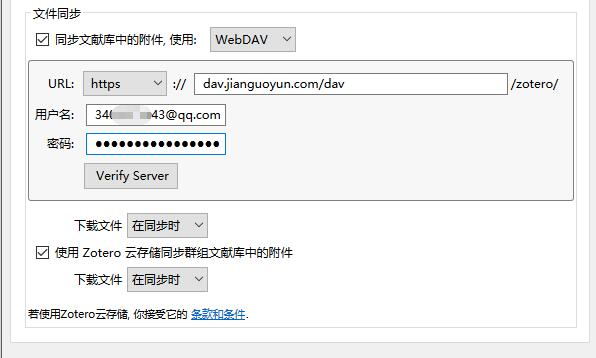
\includegraphics{./images/zotero_login.jpg}

4.下载插件 - \href{http://zotfile.com/}{ZotFile}, 用来管理PDF文件; -
\href{https://retorque.re/zotero-better-bibtex/}{Better BibTeX},
将library导出为bib.格式与RMarkdown联动。 -
\href{https://github.com/l0o0/jasminum}{Jasminum},
让Zotero更好适配知网。

下载完成后进入软件-工具-插件-设置(齿轮标识)-\texttt{Install\ Add-on\ From\ File}-安装已经下载的两个插件。

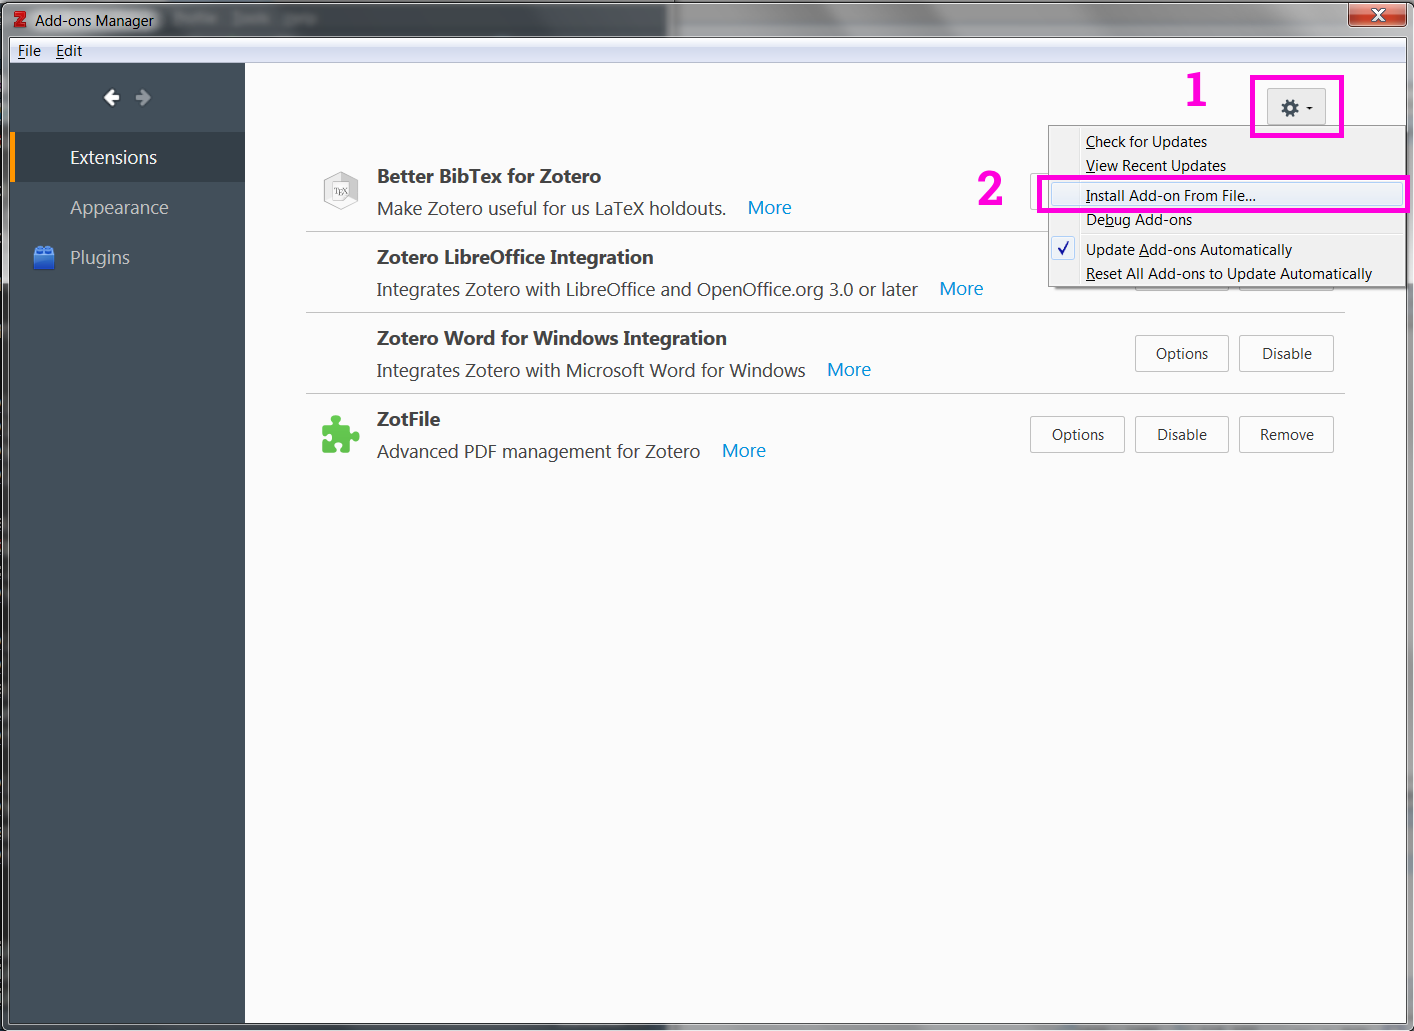
\includegraphics{./images/zotero_plugin.png}

\hypertarget{ux4feeux6539ux8bbeux7f6e}{%
\section{修改设置}\label{ux4feeux6539ux8bbeux7f6e}}

\hypertarget{ux5e38ux89c4-general}{%
\subsection{常规 general}\label{ux5e38ux89c4-general}}

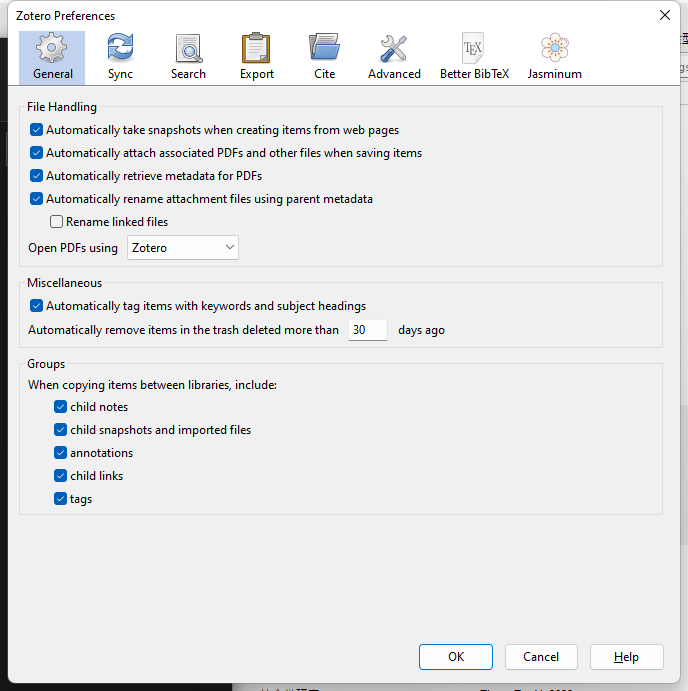
\includegraphics{./images/zotero_general.png}

\hypertarget{ux540cux6b65-sync}{%
\subsection{同步 sync}\label{ux540cux6b65-sync}}

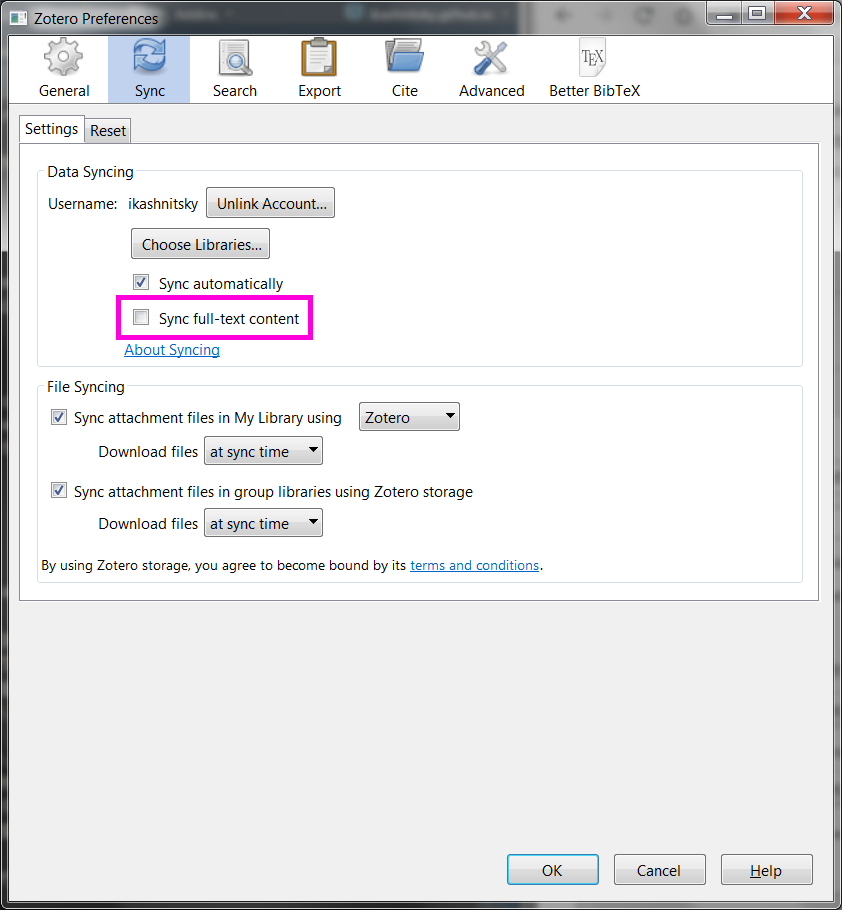
\includegraphics{./images/zotero_sync.png}

选择自动同步,取消选择{[}同步全文{]},(zotero只有300MB文件储存空间,可配置云端同步进行解决,见后文。)

\hypertarget{ux641cux7d22}{%
\subsection{搜索}\label{ux641cux7d22}}

保持默认即可。

\hypertarget{ux5bfcux51fa}{%
\subsection{导出}\label{ux5bfcux51fa}}

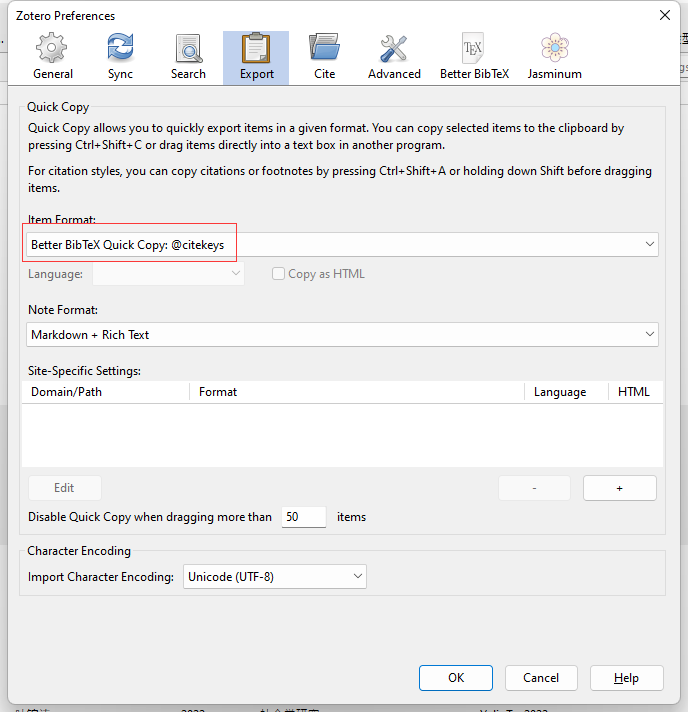
\includegraphics{./images/zotero_export.png}

\hypertarget{ux5f15ux7528}{%
\subsection{引用}\label{ux5f15ux7528}}

针对参考文献格式的设置。点击{[}获取更多样式{]}进入Zotero远程引文格式库。引文格式也可以通过.csl本地文件进行导入,点击{[}+{]}。

在''文字处理软件''(Word Processors)中安装MS Word加载项。

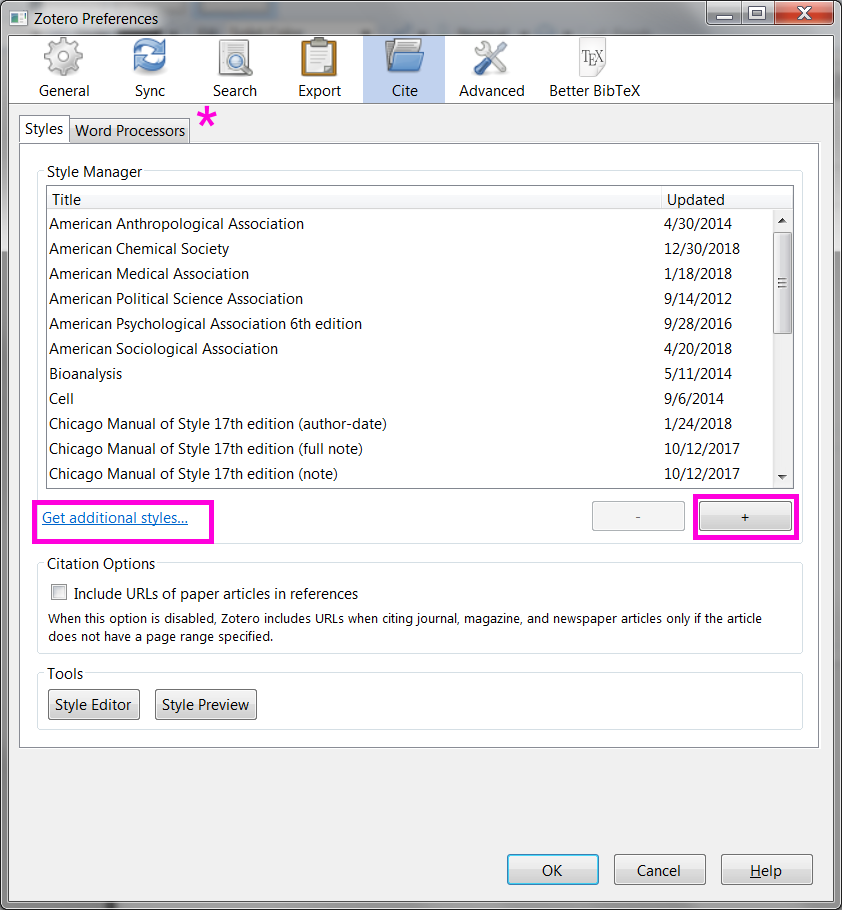
\includegraphics{./images/zotero_cite.png}

\hypertarget{sec-zotero-advanced}{%
\subsection{高级}\label{sec-zotero-advanced}}

文件储存位置:编辑-首选项-高级-文件和文件夹(Files and Folders)

设置根目录(Based directory)和数据存储位置。
根目录中存储文章的pdf文件,可酌情放在较空的硬盘中。

数据储存位置(Data directory location)仅包含Zotero中的引录信息。

后期如须多设备同步可将根目录文件夹进行云同步处理。

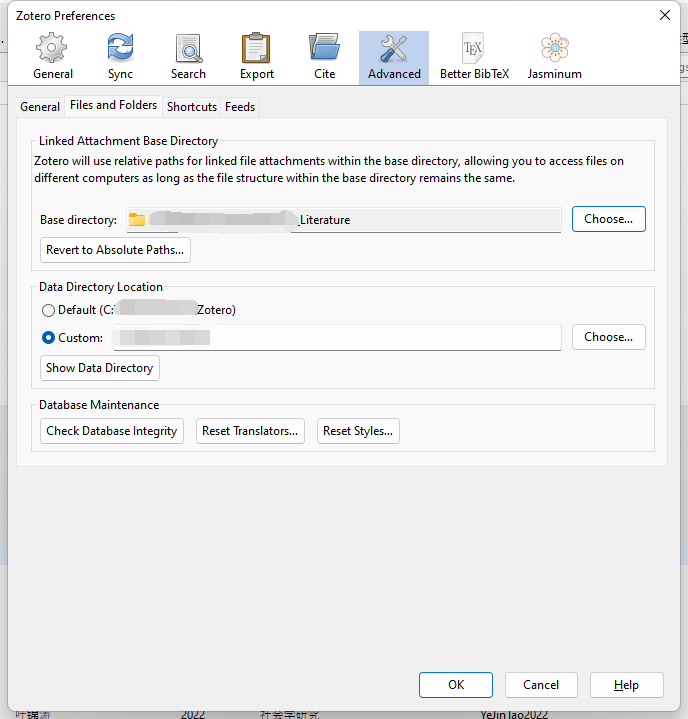
\includegraphics{./images/zotero_advanced.png}

\hypertarget{better-bibtex}{%
\subsection{Better BibTeX}\label{better-bibtex}}

在安装Better BibTeX扩展程序后,将显示此选项卡。
安装扩展将整个书目库(或其某些部分)导出为纯.bib文本文件。
在使用rmarkdown撰写学术论文时,需要此步骤才能在RStudio中使用Zotero。

变更Citation key 格式,
推荐格式\texttt{authEtAl.capitalize+year}。\footnote{更多设置详见\href{https://retorque.re/zotero-better-bibtex/citation-keys/}{cite
  key 设置查阅手册}。}

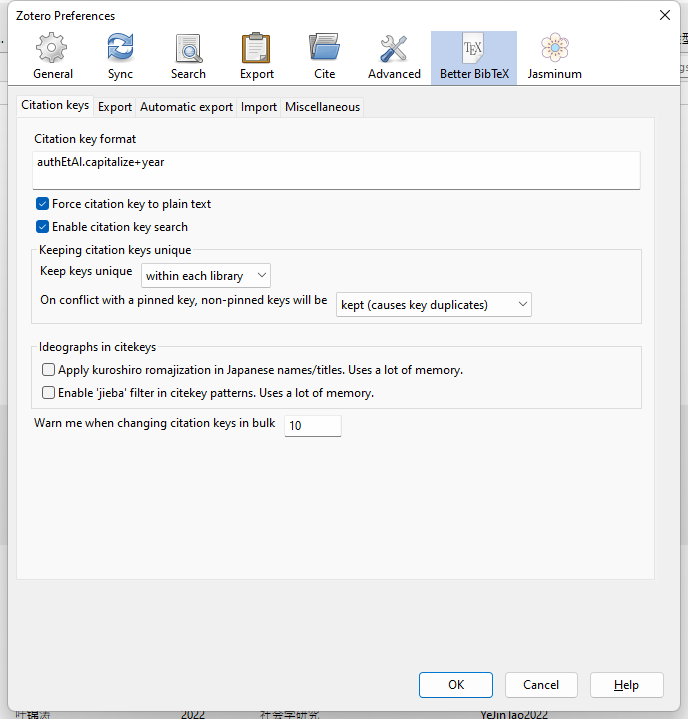
\includegraphics{./images/zotero_bibtex1.png}

自动输出(Automatic export)设置:

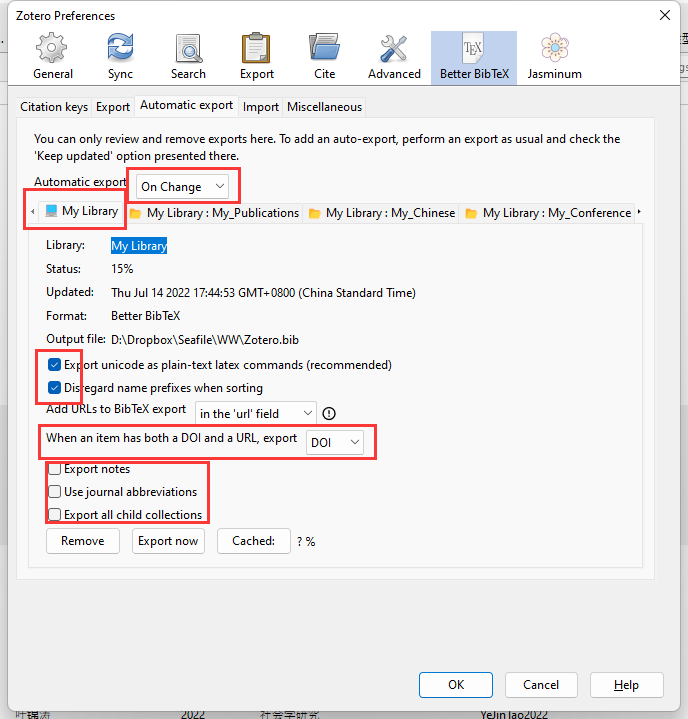
\includegraphics{./images/zotero_bibtex2.png}

\hypertarget{sec-zotero-jasminum}{%
\section{Jasminum 设置}\label{sec-zotero-jasminum}}

之前请按照提示,先安装PDFtk Server。

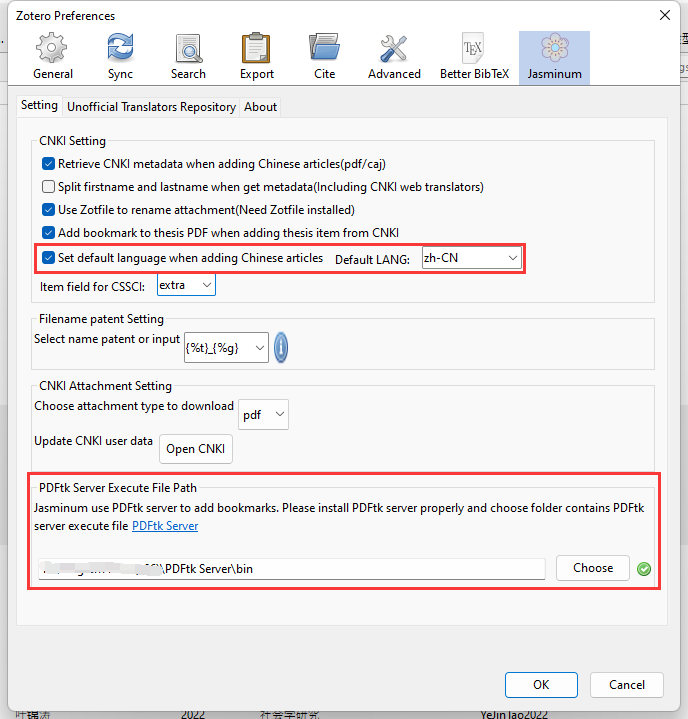
\includegraphics{./images/zotero_jasminum.png}

\hypertarget{zotfile-ux8bbeux7f6e}{%
\subsection{ZotFile 设置}\label{zotfile-ux8bbeux7f6e}}

【工具】-【ZotFile preference】

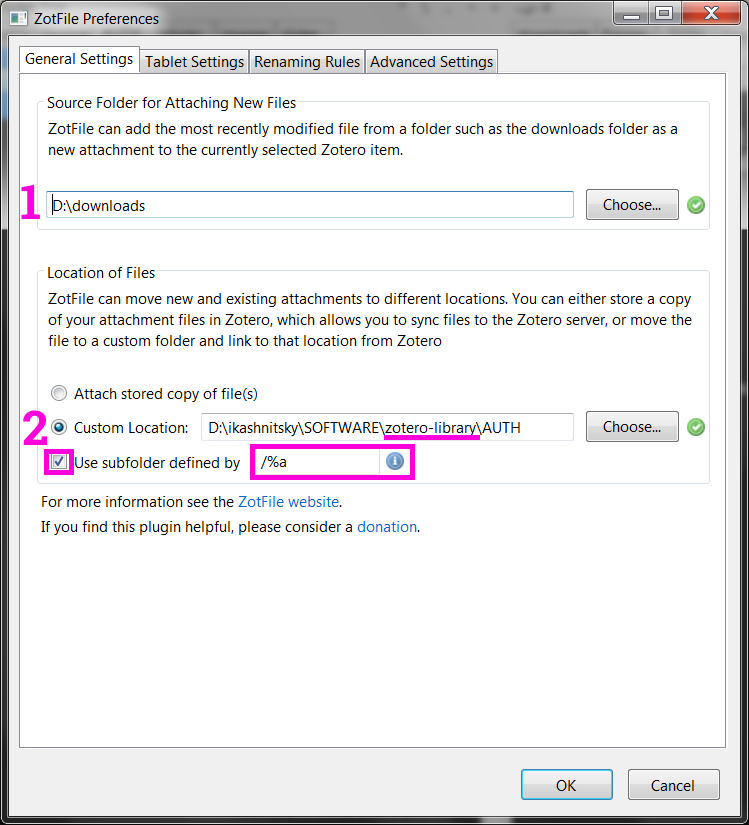
\includegraphics{./images/zotero_zotfile.png}

在这里,我们定义了两条路径。 第一个是浏览器下载的文件的默认位置。

第二条路径指向为全文PDF创建的本地目录,我将其命名为zotero-library,并与我们选择的外部云解决方案同步。

下面的use subfolder defined by
xxx的表示:根据paper的xxx来给论文分类(以再创建二级文件夹的方式)
/\%a的意思是按照作者名称分类。

\hypertarget{renaming-rules}{%
\subsection{Renaming Rules}\label{renaming-rules}}

设置附件的重命名格式, 推荐以下设置\texttt{\{\%a\}\{\%y\_\}\{\%t\}}。

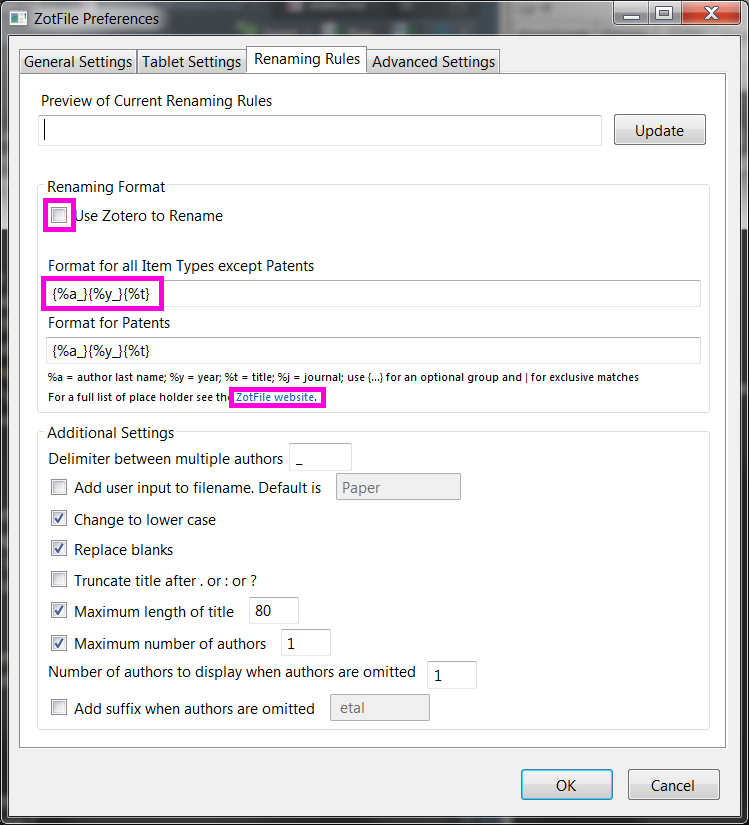
\includegraphics{./images/zotero_rename.png}

\hypertarget{ux624bux52a8ux91cdux547dux540dux9644ux4ef6}{%
\section{手动重命名附件}\label{ux624bux52a8ux91cdux547dux540dux9644ux4ef6}}

在具体的条目中点击【附件】-【重命名附件】

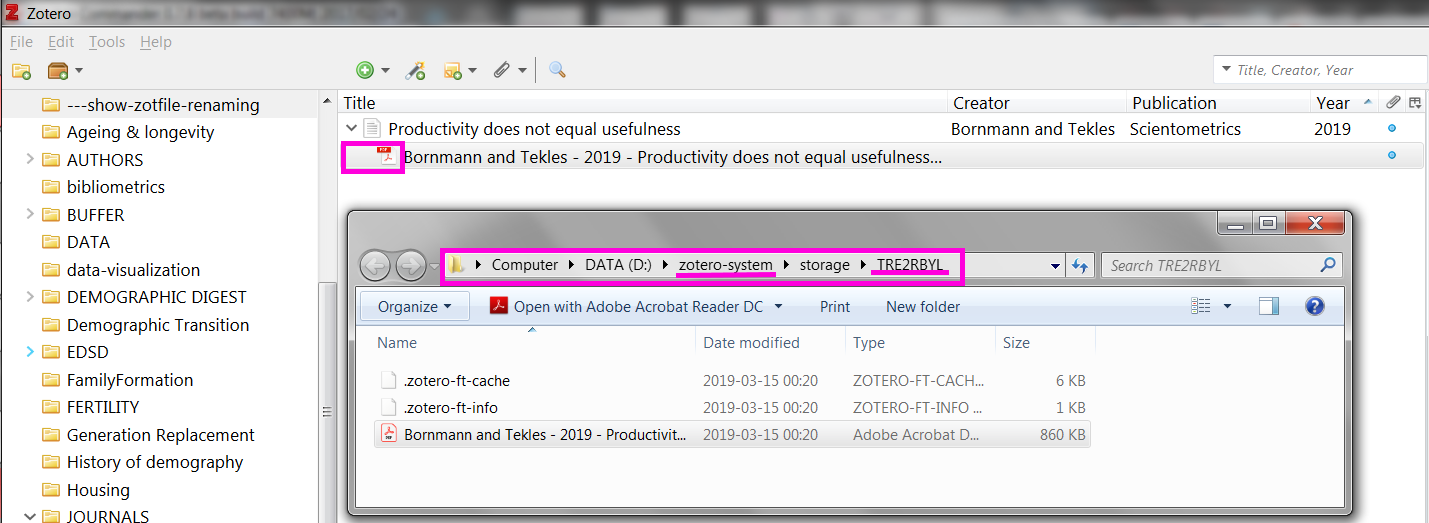
\includegraphics{./images/zotero_pdf.png}

\hypertarget{zotero-ux4e0ermarkdownux8054ux52a8}{%
\section{Zotero
与RMarkdown联动}\label{zotero-ux4e0ermarkdownux8054ux52a8}}

用插件 Better BibTeX 实现RMarkdown 中的自动引用功能。

Better
BibTeX提供了一种简便的方法,可以将Zotero的书目记录导出为纯.bib文本,并在记录更改后保持文件更新。只需右键单击Zotero中的集合,然后选择``导出集合''。

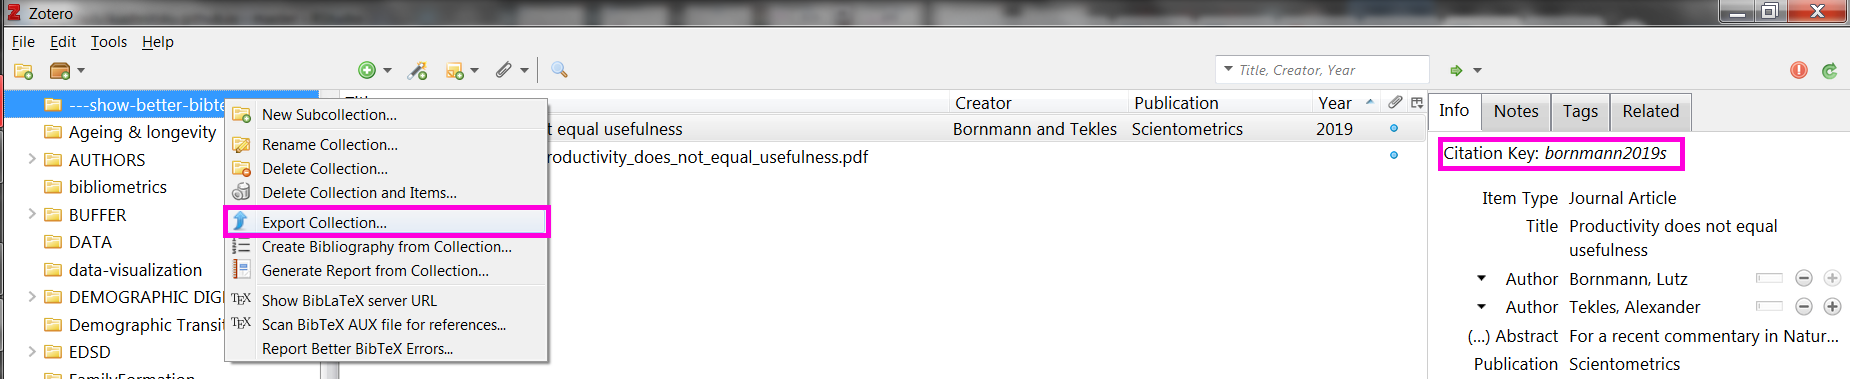
\includegraphics{./images/zotero_bbt.png}

选择持续更新。

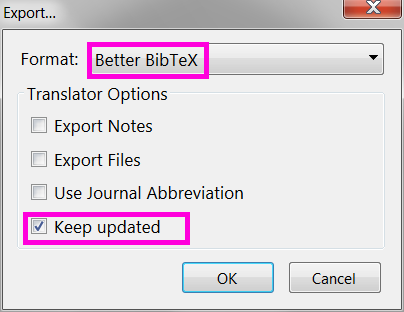
\includegraphics{./images/zotero_menu.png}

输出的.bib文件应放置在我们要编织.rmd文件的目录中。
.bib的名称在.rmd的YAML标头中指定。示例如图。

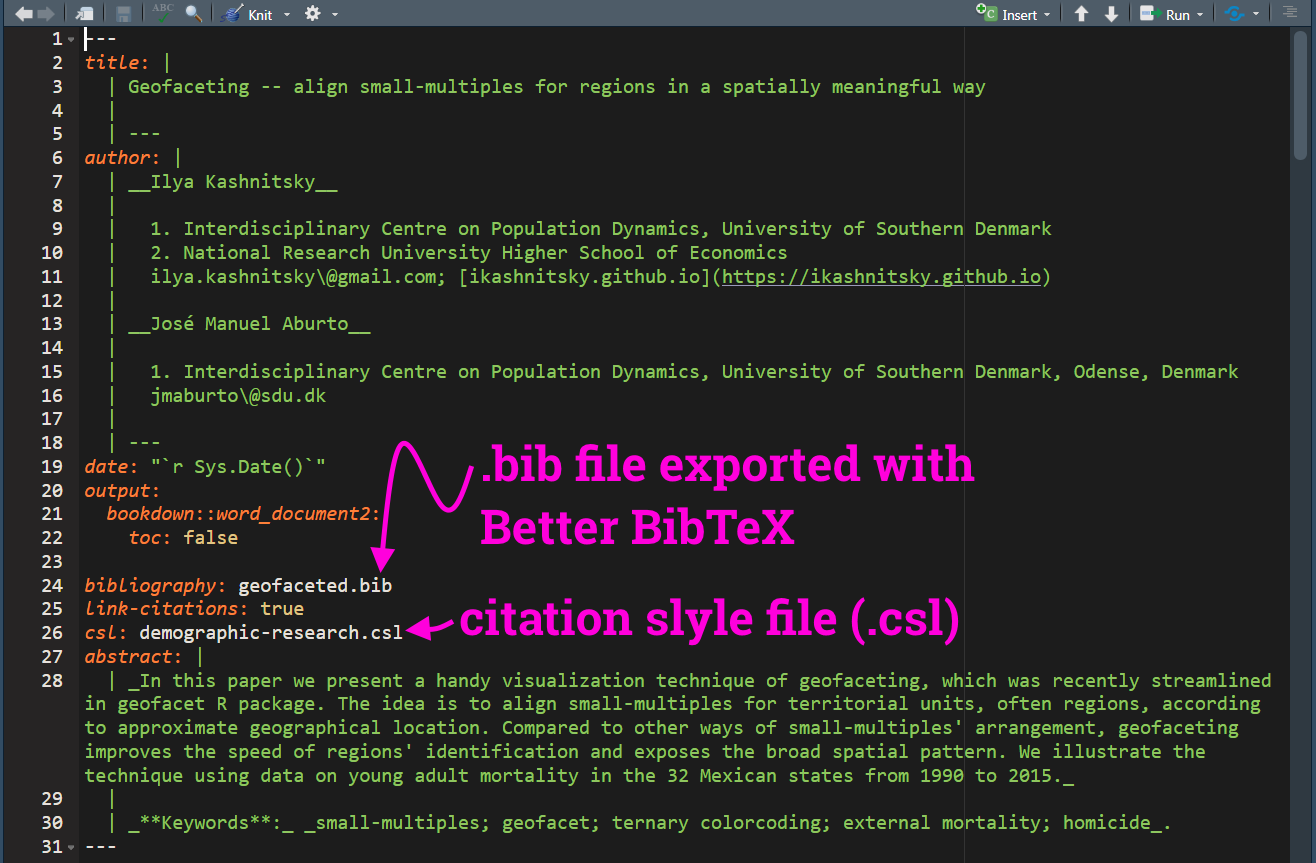
\includegraphics{./images/zotero_yaml.png}

关于R部分的更多信息请参考:

\href{https://rmarkdown.rstudio.com/authoring_bibliographies_and_citations.html}{RStudio
手册}

\href{https://bookdown.org/yihui/bookdown/citations.html}{相关章节}

或
\href{https://bookdown.org/yihui/bookdown/citations.html}{xieyihui的相关教程}

\begin{quote}
祝贺!你已经完成了设置,请奖励自己一只鸡腿!
\end{quote}

\bookmarksetup{startatroot}

\hypertarget{sec-lit}{%
\chapter{文献整理}\label{sec-lit}}

Zotero是核心文献管理工具,它不只能对文献进行归类和标签链接,同时提供了强大的文件笔记功能。
因此我们推荐将每篇文献的单独记录也在其中完成。
对于Zotero的有效设置可以参见 Chapter~\ref{sec-zotero}
中的内容,本章主要对于单篇文献笔记方法进行介绍。

\hypertarget{ux7b14ux8bb0ux5bfcux5165}{%
\section{笔记导入}\label{ux7b14ux8bb0ux5bfcux5165}}

对于笔记导入的方法,我们建议采用Zotero +
浏览器插件形式进行,避免手动输入。
安装Zotero后,会自动提示安装浏览器插件。
安装好后,第一次使用需要在插件中登录你的Zotero账号。
之后,只要插件会对各种浏览网页内容进行分类,如果是文章或者书籍信息则会自动转换图标,提示可以导入。
你只需要点击一下,就能自动导入Zotero。
如果你使用的是校园网或者校园VPN且你的图书馆购买了此资料,那么资料附件则会自动导入并存储到你之前设置的文件夹。\footnote{设置参见
  Chapter~\ref{sec-zotero} 。}

\begin{tcolorbox}[enhanced jigsaw, arc=.35mm, breakable, coltitle=black, colframe=quarto-callout-note-color-frame, toptitle=1mm, colbacktitle=quarto-callout-note-color!10!white, leftrule=.75mm, left=2mm, bottomtitle=1mm, rightrule=.15mm, title=\textcolor{quarto-callout-note-color}{\faInfo}\hspace{0.5em}{Note}, opacityback=0, bottomrule=.15mm, titlerule=0mm, opacitybacktitle=0.6, colback=white, toprule=.15mm]
注意:Zotero插件需要在Zotero本地软件打开情况下才能较好运行。
\end{tcolorbox}

通过Zotero导入笔记有几点注意事项:

\begin{enumerate}
\def\labelenumi{\arabic{enumi}.}
\tightlist
\item
  及时修补。
  Zotero随让能够帮你完成90\%的文献信息输入工作,但有时也会出现信息错漏的地方,比如原文作者可能都是用英文大写或者中文名称依旧采用姓名分开方式。
  有时也会丢失一些信息。
  这就要求使用者\emph{及时对输入信息进行检查,及时进行添改,保证信息正确}。
\item
  知网。 知网对于外部信息通常不友好。
  但这一问题很大程度上可以通过\texttt{jasminum}插件解决,请无比安装且做好设置。\footnote{参见
    Section~\ref{sec-zotero-jasminum} 。}
  安装成功后,\texttt{jasminum}选项也会出现在右键菜单中,请妥善使用。
\item
  提前分类。
  Zotero支持文献分种类、分内容保存,同时又支持全局搜索,因此请在收集文献前事先建立分类。
  建立方式和在电脑中建立文件夹类似,在此不做赘述。
\end{enumerate}

\hypertarget{ux5355ux7bc7ux7b14ux8bb0}{%
\section{单篇笔记}\label{ux5355ux7bc7ux7b14ux8bb0}}

高效读书笔记须兼备两个原则:好记和好搜。
所谓``好记''是指能够快速的将文章内容和重点理清,当回看笔记的时候也能快速定位到需要的部分。
所谓``好搜''是指在记录笔记时即考虑到日后搜索的需要,重视关键字和短语的记录。

基于以上原则,我推崇使用结构化笔记方式来记录单篇文献,即对文章各部分内容进行拆解,填充到固定的笔记分节中去。
这里介绍的方式,是我和我组成员长期实践的结果。其中分节设置部分借鉴了\emph{Social
Science Quarterly}的摘要写作方式,总体包含五部分:

\begin{enumerate}
\def\labelenumi{\arabic{enumi}.}
\tightlist
\item
  Objective:文章主要研究对象,一般能在题目和摘要中找到。

  \begin{itemize}
  \tightlist
  \item
    推荐将文中一些重要概念也记录到这部分。
  \end{itemize}
\item
  Theory: 文章的主要观点、理论逻辑等。
\item
  Method:采用的研究方法。

  \begin{itemize}
  \tightlist
  \item
    如果是理论性文章Method部分可省略。
  \item
    如果是实证性文章,请记录以下内容:

    \begin{enumerate}
    \def\labelenumii{\arabic{enumii}.}
    \tightlist
    \item
      Data:数据来源、体量、搜集过程等信息
    \item
      Method:数据分析方法、重要方法决定、稳健性检验等
    \end{enumerate}
  \end{itemize}
\item
  Findings:文章的主要发现,本部分业主要针对实证文章
\item
  Highlights:文章的亮点

  \begin{itemize}
  \tightlist
  \item
    Lits: 文中提及的可能以后会用到的一些文献综述
  \item
    Theory:文章一些理论观点或者未来理论可以生发之处
  \item
    Method: 文中提到的一些方法方面的综述或者讨论
  \item
    Empirics:文中提及的其他文章中的实证发现
  \item
    Wording:高效、地道的中英文词汇
  \end{itemize}
\end{enumerate}

在记录这些内容的过程中,请尽量使用短语、bullet points,
箭头等形式,避免大段摘抄。 另外Zotero有强大的文本标注和转化功能。
你可以在阅读过程中即对文本进行分类标注,然后转化成上述笔记形式。

\hypertarget{ux7b14ux8bb0ux5171ux4eab}{%
\section{笔记共享}\label{ux7b14ux8bb0ux5171ux4eab}}

Zotero能很好支持线上和线下文献共享。
我们推荐采用线下共享方式,以保证本地端包含文献的记录、笔记、文档等所有内容。
导出方式非常简单,只需选中需要文本,右键选择导出。

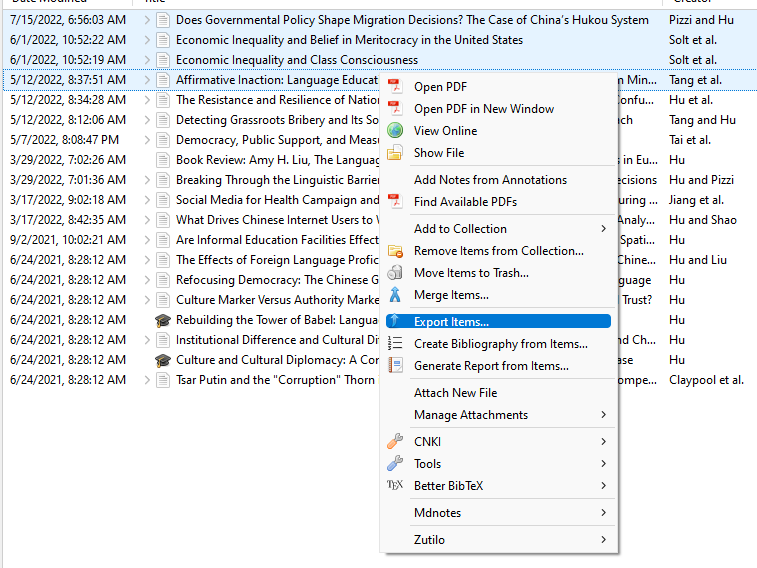
\includegraphics{./images/lit_export.png}

之后在导出项中选择\texttt{Zotero\ RDF}格式,然后勾选导出笔记、文件和标注。
生成文件将是一个包含了文献文本和\texttt{.rdf}的文件夹,压缩后分享给同伴即可。
我们推荐对多个文献采用多选分享方式,而不是一篇文章一个rdf。

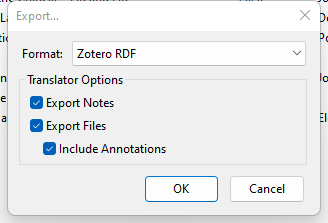
\includegraphics{./images/lit_export_set.png}

\bookmarksetup{startatroot}

\hypertarget{sec-rmarkdown}{%
\chapter{Rmarkdown}\label{sec-rmarkdown}}

Rmarkdown是markdown的一种延伸版本。
Markdown是一种流行且轻量级的标记语言。
标记语言旨在将文本内容和结构(比如各级标题、链接、表格、图片、脚注等)结合展现的文本书写方式。
在\texttt{Pandoc}的帮助下,markdown语言能够轻松地实现html、pdf或docx文本输出。
这方面你可能听说过一个很强大的排版软件,LaTex。
在很多人看来(包括我),markdown语言很大程度上能够替代LaTex。
他们都能生成pdf(事实上markdown是通过\texttt{Pandoc}撰写成tex文件,所以本质上是一回事),而markdown的学习门槛和书写结果都比LaTex友好得多。

本节的核心目的是教会你如何使用rmarkdown进行学术论文写作。
使用进行学术写作的优点有四:

\begin{enumerate}
\def\labelenumi{\arabic{enumi}.}
\tightlist
\item
  保证分析和文字都在同一个文档中,避免忘记code对应什么内容的情况;
\item
  自动生成Replication file,
  任何人拿到文件后都能够得出和作者一致的结果,最大程度上实现研究透明;
\item
  能轻松导出html,MS word, 或pdf文档,适应中英文写作各种要求。
\item
  很好兼容Git版本控制。
\end{enumerate}

\hypertarget{yaml-ux8bbeux7f6e}{%
\section{YAML 设置}\label{yaml-ux8bbeux7f6e}}

Rmarkdown写作的第一步应该是设置YAML。 所谓YAML,是``Yet Another Markup
Language''的缩写,通常用作全篇样式的设置,写在每篇文章的最开始的位置。
以下是我和我的合作者在\emph{Chinese Journal of International
Politics}上发表的``The Resistance and Resilience of National Image
Building: An Empirical Analysis of Confucius Institute Closures in the
U.S.''一文的YAML设置。\footnote{ Hu, Yue, Yufei Sun, and Donald Lien.
  2022. ``\href{https://10.1093/cjip/poac010}{The Resistance and
  Resilience of National Image Building: An Empirical Analysis of
  Confucius Institute Closures in the U.S.}'' \emph{Chinese Journal of
  International Politics} 15(3): 1--18.} 我们将逐步介绍其中的设置:

\begin{verbatim}
---
output: 
  bookdown::pdf_document2:
    fig_caption: true
    number_sections: true

fontsize: 12pt
indent: true
geometry: margin=1in
bibliography: Zotero.bib
csl: chinese-journal-of-international-politics.csl
link-citations: true
colorlinks: true
toc: false

title: 'Resistance and Resilience: A Study of National Image Building Based on Confucius Institute Closures in the U.S.'

author:
- Yue Hu^[Tsinghua University]
- Yufei Sun^[Tsinghua University, Corresponding Author]
- Donald Lien^[University of Texas at San Antonio]

abstract: |
  National image building (NIB) has become a critical strategy in public diplomacy.
  Extending the existing sender-focused literature on NIB, this study takes the receiver side into account.
  Focusing on the closures of a critical NIB effort of China, Confucius Institutes (CIs) in the U.S., we examine how a powerful receiver's resistance affect the image of the sender domestically.
  Based on an extensive dataset of American CIs, we also dig in who exactly in the receiver country promote the resistance.
  The analytic results shows that the CI closures turn down both media tone of and attention to China in the U.S. but locally at most.
  Meanwhile, the empirical evidence also support the resilience of NIB: the remaining CIs still improve local image of China; even in places no CIs left openning, the media attention to China is still higher.
  There are also evidence for the resilience of the NIB efforts: the remaining CIs still improve the media image of China.
  Regarding the promoters of NIB resistance, American colleges show a certain level of autonomy on the CIs' fate; the government has an influence on the issue yet largely through affecting public schools' decisions.
  
  **Keywords:** National image, public diplomacy, Confucius Institutes, U.S-China relations, soft power, GDELT.
---
\end{verbatim}

\begin{itemize}
\tightlist
\item
  \texttt{output}:用于设置文章的输出类型。
  如前所述,\texttt{rmarkdown}可以输出html、pdf或docx三种类型,这里是确定输出格式的地方。

  \begin{itemize}
  \tightlist
  \item
    \texttt{bookdown::pdf\_document2}:在上面的例子里,我们设置输出格式为pdf,这也是国际期刊投稿的常见格式。
  \item
    \texttt{fig\_caption:\ true}:这里表示我们希望文章中显示图片的标题。
  \item
    \texttt{number\_sections:\ true}:这里表示我们希望文中标题显示编号。有的期刊可能会有不允许章节编号的要求,此时将\texttt{true}变成\texttt{false}即可。
  \end{itemize}
\end{itemize}

\begin{tcolorbox}[enhanced jigsaw, arc=.35mm, breakable, coltitle=black, colframe=quarto-callout-tip-color-frame, toptitle=1mm, colbacktitle=quarto-callout-tip-color!10!white, leftrule=.75mm, left=2mm, bottomtitle=1mm, rightrule=.15mm, title=\textcolor{quarto-callout-tip-color}{\faLightbulb}\hspace{0.5em}{Bookdown输出格式}, opacityback=0, bottomrule=.15mm, titlerule=0mm, opacitybacktitle=0.6, colback=white, toprule=.15mm]
\texttt{bookdown}中提供了\texttt{pdf\_document}和\texttt{pdf\_document2}两种格式,都可以输出pdf,但后者支持相互参照(cross
reference),这个我们之后会讲到。
\end{tcolorbox}

\begin{itemize}
\tightlist
\item
  段落格式

  \begin{itemize}
  \tightlist
  \item
    \texttt{fontsize:\ 12pt}:字体大小,\texttt{12pt}是英文发表的标准字体大小
  \item
    \texttt{indent:\ true}:采用每段空两格格式,如果\texttt{false}则采用每段顶格,段间空行模式
  \item
    \texttt{geometry:\ margin=1in}:每页边距1 inch
  \item
    \texttt{bibliography:\ Zotero.bib}:为参考文献文件,最方便的是使用Zotero生成,将在
    Chapter~\ref{sec-zotero} 详细讲解。
  \item
    \texttt{csl:\ chinese-journal-of-international-politics.csl}:\href{https://citationstyles.org/}{Citation
    Style Language
    (CSL)}用于自动设置参考文献格式。换言之,只要你使用rmarkdown就再也不需要手动更改参考文献,只需要找到的对应期刊的\texttt{.csl}文件即可。
  \item
    \texttt{link-citations:\ true}:将文中所有引用加入超链接,直接对应最后的参考文献列表的对应位置。
  \item
    \texttt{colorlinks:\ true}:文中超链接采用不同颜色
  \item
    \texttt{toc:\ false}:``table of
    content''(toc),即目录。通常文章不需要目录,因此我们选择否。
  \end{itemize}
\item
  首页

  \begin{itemize}
  \tightlist
  \item
    \texttt{title}:文章标题,如果需要副标题,可加\texttt{subtitle}选项。
  \item
    \texttt{author}:作者
  \item
    \texttt{abstract}:摘要和关键字。
  \end{itemize}
\end{itemize}

\hypertarget{ux6b63ux6587ux8bbeux7f6e}{%
\section{正文设置}\label{ux6b63ux6587ux8bbeux7f6e}}

\begin{verbatim}
National image building (NIB) is the efforts of a country to improve the public impressions of and attitudes towards it in a receiver country.
Sender countries commonly expect the NIB efforts to bring better acceptance of their people, products, and investments in the receiver country. 
While NIB has become widely practiced around the world regardless of the country's size or power, there has not been a consensus about its effect. [@Barr2012;@OwenIV2010;@LienEtAl2012;@XiePage2013;@LiEtAl2014;@BrazysDukalskis2019b;@Meng2020]......

# Building National Image: Source, Function, and Effects

......

# Examining NIB Resistance-Resilience Based on CI Closures in the U.S. 

## Data Generation Process
\end{verbatim}

一般学术论文正文最多使用三级标题,可如上例使用1\textasciitilde3个\#标识。
个数越多,标题层级越低。
\texttt{{[}@xxx{]}}为生成引文,其生成格式由Zotero内Bibtex生成的Citekey决定,将在
Chapter~\ref{sec-zotero} 部分详细讲解。
此外,除文字外,Rmarkdown还插入代码块、图表等其他内容,可参见\href{https://bookdown.org/yihui/rmarkdown/r-code.html}{R
Markdown: The Definitive Guide}相关内容。

\hypertarget{ux4e2dux6587ux8bbaux6587ux5199ux4f5c}{%
\section{中文论文写作}\label{ux4e2dux6587ux8bbaux6587ux5199ux4f5c}}

不论是在学校上学还是在国内做研究,Microsoft Word是必用工具。
Rmarkdown可以非常方便地生成docx文档,使你几乎不用再打开Word------以及忍受闪退、格式不统一等Word弊病------实证研究和实证写作的真正融合。

使用Rmakrdown进行Word写作基本步骤和上面完全一样,唯一需要调整的是YAML部分。
以下以我和朱萌在《治理研究》发表的``以语塑心与国民治理:外语习得对政治认知能力的塑造机制研究''的YAML为例进行研究。\footnote{胡悦
  and 朱萌. 2022.
  ``以语塑心与国民治理:外语习得对政治认知能力的塑造机制研究.''
  《治理研究》38(4): Online.}
比起之前的例子,最主要的改变是在\texttt{output}部分从\texttt{bookdown::pdf\_document2:}变为\texttt{bookdown::word\_document2}。
另一个改变重点是\texttt{reference\_docx:\ template\_cn.docx}。由于中文期刊往往有一些特殊的设置要求包括章节号、段落缩进、字体等等,这些都可以通过\texttt{template\_cn.docx}以MS
Word template方式进行调试。
详细的设置方式可以参考以下两个资源:\href{https://bookdown.org/yihui/rmarkdown-cookbook/word-template.html}{R
Markdown
Cookbook}和\href{https://bookdown.org/yihui/bookdown/internationalization.html}{Authoring
Books with R Markdown}。

\begin{verbatim}
--
output:
  bookdown::word_document2:
    number_section: false
    reference_docx: template_cn.docx
fontsize: 12 pt
geometry: margin=1in
bibliography:  "language_English.bib"
csl: "american-political-science-review.csl"
link-citations: true
colorlinks: false

title: |
  以语塑心与国民治理:外语习得对政治认知能力的塑造机制研究
author: 
- 胡悦
- 朱萌^[胡悦,清华大学政治学系副教授;朱萌,通讯作者,清华大学政治学系硕士研究生。**基金项目**:国家自然科学基金委青年项目“新型城镇化进程中新老市民身份认同建构的社会心理机制与政策引导路径研究”(72004109),清华大学自主科研项目“新时代国民身份认同建构机制研究”(2019THZWJC47)。]

abstract: |

 **摘要**:
 掌握外语人口增加是现代化发展在个体层面的重要特征,也是一国站稳国际舞台、引领世界潮流的重要前提。
 然而,现有研究多聚焦外语的对外功能和教育手段,对其对内功用,尤其是社会政治功用和治理价值却不甚明了。
 “语言政策场域”理论结合语言治理和语言政治学逻辑填补此方面空白,指出外语习得对国民政治能力(特别是以政治效能感为代表的政治感知能力)的提升效果以及四种作用机制。
 基于全国代表性样本的实证分析支持了该理论的效果和机制假设。
 实证研究表明,中国国民外语(英语)水平对其政治认知能力具有显著促进作用。
 在机制上,外语习得通过信息获取进路上提升内部政治效能感作用最明显,而语言竞争优势则是影响外部效能感的主导路径。
 与此同时,价值西化路径并未对国民政治认知造成明显改变。
 据此,外语习得对于国民政治能力塑造功能更偏向素质性,而非价值性。
 对于语言政策场域理论的系统探讨和实证检验推进了对宏观语言政策微观治理逻辑的理解,为“语言--思维”关系这一经典议题提供新思路和新证据,同时对于像中国这样外语人口日益庞大的现代国家治理也具有重要现实意义,为我国改革语言政策和治理体系、提升国家能力、推动国家治理现代化提供理论借鉴和实证参考。
 
 **关键词**:国家治理能力;政治能力;语言治理;外语习得;政策场域;政治效能感。
 
 Foreign Language and Governance: How Second Language Acquisition Constructs Mass Cognitive Capability for Politics
 
 **Abstract**:The growth of the population comprehending a second language is a characteristic of modernization and the prerequisite of a state's international influence. 
 However, the mainstay of the existing research on second language acquisition (SLA) focuses on international communications and education ignoring SLA's sociopolitical functions and values for domestic governance.
 The novel "language policy field" theory fills this academic vacuum by specifying four paths SLA can affect individuals' political capabilities, especially the cognitive capability. 
 The study based on a nationally representative survey in China supports the hypotheses of this theory. 
 The empirical analyses show that Chinese citizens' English proficiency significantly modifies people's cognitive capability of politics as measured by political efficacy. 
 In terms of the mechanisms, SLA increases the internal efficacy mainly through the information-collection mechanism while raising the external efficacy through the relative-proficiency mechanism. 
 Meanwhile, there is no evidence that SLA affects political capacities through value changes. 
 In this sense, the influence of SLA is more on literacy than on beliefs. 
 The new theory and findings have far-reaching implications on language governance, national capacity, and the modernization of governance in general.
 
 **Keywords**:National capacity of governance; political capacity; language governance; second-language acquisition (SLA); policy field; political efficacy.

---
\end{verbatim}

\bookmarksetup{startatroot}

\hypertarget{sec-bookdown}{%
\chapter{Bookdown}\label{sec-bookdown}}

Bookdown是\texttt{rmarkdown}的一个重要延伸,我们在
Chapter~\ref{sec-rmarkdown} 中已经使用到了这一软件。
然而,如名所示,bookdown的本业是写书。
因此使用Bookdown撰写学位论文能将\texttt{rmarkdown}的所有优势都能充分利用,并最大限度减少文献整理等无效工作。\footnote{本章写作获得了石宇洋同学很大帮助。}

以下对和学术写作相关的Bookdown设置进行介绍。

\hypertarget{bookdownux5305ux4e0bux8f7d}{%
\section{Bookdown包下载}\label{bookdownux5305ux4e0bux8f7d}}

\begin{Shaded}
\begin{Highlighting}[]
\FunctionTok{install.packages}\NormalTok{(}\StringTok{\textquotesingle{}bookdown\textquotesingle{}}\NormalTok{)}

\CommentTok{\# or Github}

\NormalTok{devtools}\SpecialCharTok{::}\FunctionTok{install\_github}\NormalTok{(}\StringTok{\textquotesingle{}rstudio/bookdown\textquotesingle{}}\NormalTok{)}
\end{Highlighting}
\end{Shaded}

\hypertarget{bookdown-projectux5373ux4f60ux7684ux5b66ux4f4dux8bbaux6587ux7ed3ux6784}{%
\section{Bookdown
Project(即你的学位论文)结构}\label{bookdown-projectux5373ux4f60ux7684ux5b66ux4f4dux8bbaux6587ux7ed3ux6784}}

请在进行Bookdown书写时,首先创建一个新的project。Working
directory中一般有以下部分:

\texttt{index.Rmd}: Rmd的第一章节,包括整本书的格式设置和第一章内容

\texttt{num-name.Rmd}:\texttt{num}决定\texttt{Bookdown}输出时的章节顺序,保序;\texttt{name}自己起名

\texttt{\_bookdown.yml}:输出格式逻辑调整,一般不用

\texttt{\_output.yml}:输出格式内容调整(例如书名),一般只需要更改全书书名

\texttt{preamble.tex}和\texttt{style.css}:Latex和Css调整输出样式

其他可能还有\texttt{.bib}(引用,见Zotero部分)。

\begin{Shaded}
\begin{Highlighting}[]
\NormalTok{directory}\SpecialCharTok{/}
\NormalTok{├──  index.Rmd}
\NormalTok{├── }\DecValTok{01}\SpecialCharTok{{-}}\NormalTok{intro.Rmd}
\NormalTok{├── }\DecValTok{02}\SpecialCharTok{{-}}\NormalTok{literature.Rmd}
\NormalTok{├── }\DecValTok{03}\SpecialCharTok{{-}}\NormalTok{method.Rmd}
\NormalTok{├── }\DecValTok{04}\SpecialCharTok{{-}}\NormalTok{application.Rmd}
\NormalTok{├── }\DecValTok{05}\SpecialCharTok{{-}}\NormalTok{summary.Rmd}
\NormalTok{├── }\DecValTok{06}\SpecialCharTok{{-}}\NormalTok{references.Rmd}
\NormalTok{├── \_bookdown.yml}
\NormalTok{├── \_output.yml}
\NormalTok{├──  book.bib}
\NormalTok{├──  preamble.tex}
\NormalTok{├──  README.md}
\NormalTok{└──  style.css}
\end{Highlighting}
\end{Shaded}

\hypertarget{index.rmd}{%
\section{\texorpdfstring{\texttt{Index.Rmd}}{Index.Rmd}}\label{index.rmd}}

\texttt{Index.Rmd}是Bookdown中最重要的部分,其包括一个YAML和第一章内容,其中,YAML决定全书格式

\begin{Shaded}
\begin{Highlighting}[]
\SpecialCharTok{{-}{-}{-}}
\NormalTok{title}\SpecialCharTok{:} \StringTok{"Summer RA Conclusion"}
\NormalTok{author}\SpecialCharTok{:} \StringTok{"Yuyang Shi, Yokia Xu"}
\NormalTok{date}\SpecialCharTok{:} \StringTok{"\textasciigrave{}r Sys.Date()\textasciigrave{}"}
\NormalTok{site}\SpecialCharTok{:}\NormalTok{ bookdown}\SpecialCharTok{::}\NormalTok{bookdown\_site}
\NormalTok{output}\SpecialCharTok{:}\NormalTok{ bookdown}\SpecialCharTok{::}\NormalTok{gitbook}
\NormalTok{description}\SpecialCharTok{:} \StringTok{"Summer RA Conclusion"}
\NormalTok{documentclass}\SpecialCharTok{:}\NormalTok{ book}
\NormalTok{bibliography}\SpecialCharTok{:}\NormalTok{ law}\SpecialCharTok{{-}}\NormalTok{and}\SpecialCharTok{{-}}\NormalTok{politics.bib,}
\NormalTok{biblio}\SpecialCharTok{{-}}\NormalTok{style}\SpecialCharTok{:}\NormalTok{ apalike}
\SpecialCharTok{{-}{-}{-}}
\end{Highlighting}
\end{Shaded}

其中,site和output决定全书输出格式,可参见详见\href{https://bookdown.org/}{Bookdown}文档。一般而言,只需要更改\texttt{title},\texttt{author},\texttt{description},\texttt{bibliography}和\texttt{biblio-style}。

\hypertarget{num-name.rmd}{%
\section{\texorpdfstring{\texttt{Num-name.Rmd}}{Num-name.Rmd}}\label{num-name.rmd}}

在随后的所有Rmd文件中,我们只需要使用markdown语法格式进行书写即可。(安利一下Typora!)

所有的\texttt{Num-name.Rmd}都\textbf{必须包含一个一级标题},如\texttt{\#\ Bookdown}。

为组织文章结构,我们可以在每个\texttt{Num-name.Rmd}中使用任意的二级、三级标题。但请不要使用四级及以下的标题

\hypertarget{bookdown.yml}{%
\section{\texorpdfstring{\texttt{\_bookdown.yml}}{\_bookdown.yml}}\label{bookdown.yml}}

一般不使用,可以用\texttt{\_bookdown.yml}限定输出\texttt{.Rmd}的范围和顺序,如

\begin{Shaded}
\begin{Highlighting}[]

\NormalTok{rmd\_files}\SpecialCharTok{:}\NormalTok{ [}\StringTok{"index.Rmd"}\NormalTok{, }\StringTok{"02{-}git.Rmd"}\NormalTok{, }\StringTok{"01{-}Rmd.Rmd"}\NormalTok{]}
\end{Highlighting}
\end{Shaded}

将使Bookdown先输出\texttt{02-git.Rmd},再生成\texttt{01-Rmd.Rmd},且不输出其他内容。

\hypertarget{output.yml}{%
\section{\texorpdfstring{\texttt{\_output.yml}}{\_output.yml}}\label{output.yml}}

一般不使用,可以调整输出格式。详见\href{https://bookdown.org/yihui/rmarkdown/bookdown-output.html}{R
Markdown: The Definitive Guide Chapter 12.4}

\begin{Shaded}
\begin{Highlighting}[]
\NormalTok{bookdown}\SpecialCharTok{::}\NormalTok{gitbook}\SpecialCharTok{:}
\NormalTok{  lib\_dir}\SpecialCharTok{:}\NormalTok{ assets}
\NormalTok{  split\_by}\SpecialCharTok{:}\NormalTok{ section}
\NormalTok{  config}\SpecialCharTok{:}
\NormalTok{    toolbar}\SpecialCharTok{:}
\NormalTok{      position}\SpecialCharTok{:}\NormalTok{ static}
\NormalTok{bookdown}\SpecialCharTok{::}\NormalTok{pdf\_book}\SpecialCharTok{:}
\NormalTok{  keep\_tex}\SpecialCharTok{:}\NormalTok{ yes}
\NormalTok{bookdown}\SpecialCharTok{::}\NormalTok{html\_book}\SpecialCharTok{:}
\NormalTok{  css}\SpecialCharTok{:}\NormalTok{ toc.css}
\end{Highlighting}
\end{Shaded}

\hypertarget{ux8865ux5145ux8bf4ux660e}{%
\section{补充说明}\label{ux8865ux5145ux8bf4ux660e}}

\begin{enumerate}
\def\labelenumi{\arabic{enumi}.}
\item
  Bookdown中,各章节需要依照``num-name.Rmd''的方式命名。其中num决定章节先后顺序,保序即可。
\item
  Bookdown中的Zotero引用与第三部分完全一致。
\item
  即使没有''\_bookdown.yml''和''\_output.yml''文件,Bookdown依然能按照default格式输出。但在与Github连接不稳定时,将上述文件储存在本地是有用的。
\item
  在完成Bookdown各章节书写后,需要分别knit才能得到完整文档(仅knit\texttt{index.Rmd}会有各章节目录,但不会有具体内容)。
\end{enumerate}

\bookmarksetup{startatroot}

\hypertarget{ux7248ux672cux63a7ux5236}{%
\chapter{版本控制}\label{ux7248ux672cux63a7ux5236}}

本部分主要介绍版本控制(version
control),旨在对版本迭代间进行跟踪记录。
一方面,避免本地存储过多重复版本,另一方面,对文件迭代进行细致的辨析。
一定程度上,版本控制还能补全使用rmarkdown无法做修改标记的缺陷。

这个技术非常有用,但需要一段时间上手。
这里的介绍大体遵循Jenny的这本英文手册:
\href{https://happygitwithr.com/}{Get started with GitHub \textbar{}
Happy Git and GitHub for the useR}\footnote{本章写作获得石宇洋同学很大帮助。}

\hypertarget{ux7248ux672cux63a7ux5236ux8fdcux7a0bux5e73ux53f0}{%
\section{版本控制远程平台}\label{ux7248ux672cux63a7ux5236ux8fdcux7a0bux5e73ux53f0}}

版本控制在代码写作中非常常见。
最流行的控制平台当然是\href{https://github.com/}{GitHub}。
和它近似的还有Gitlab, gitee等。
清华大学也有自己的代码管理平台,根据域名推断很大可能就是假设在Gitlab上的。
使用这些平台多数时候需要首先注册账号。

\hypertarget{ux540dux8bcdux89e3ux91ca}{%
\section{名词解释}\label{ux540dux8bcdux89e3ux91ca}}

为了之后更好理解后面内容,这里要先进行几个名词解释:

\begin{itemize}
\tightlist
\item
  Git:是专门进行版本控制的软件。版本控制的大部分工作是可以在本地完成的。只需到\href{https://git-scm.com}{Git官网}下载对应版本软件、安装,即可在本地实现版本控制。但是,由于基于本地的版本控制很容易由于本地电脑问题损坏、丢失,而且也不利于团队共享和合作,因此,大量版本控制使用者更倾向于基于平台实现远程(remote)版本控制。

  \begin{itemize}
  \tightlist
  \item
    \texttt{Add}: 确定哪些命令要在一轮版本控制中进行追踪。
  \item
    \texttt{Commit}: 将新版本正式送入版本追踪序列。
  \item
    \texttt{Push}: 将新版本推到版本追踪序列中。
  \item
    \texttt{Diff}: 比较两个版本差别。
  \item
    \texttt{Pull}:
    如果多人合作,别人\texttt{push}了最新版本,你可以通过\texttt{pull}的方式把这个版本拉出来,下载到本地。
  \end{itemize}
\end{itemize}

想象一下,一个版本追踪就是将同一个文件放到专属这个文件的一个抽屉柜里,这个柜子有很多层,越往下层,版本越旧,越往上层越新。
而这个抽屉柜有个特别的功能,就是柜子每两层之间的隔板可以变透明。
所以从上往下看时候就能透过最新的对比到旧的,看出新旧的差别来。
在这个过程中,将想要追踪的的版本调出来就叫做\texttt{add},放到抽屉里叫做\texttt{commit},把抽屉进去的动作就是\texttt{push}。
对比两层的动作叫做\texttt{diff}
而把别人放进去的最新一层拿出来就叫做\texttt{pull}。

\begin{itemize}
\tightlist
\item
  Repository:如果每个文件就是一个抽屉柜,那么这些抽屉柜的总和就是一个``库'',通常简写为''repo''。
\item
  Main/branch:版本控制支持树的概念,类似\href{https://en.wikipedia.org/wiki/Multiverse}{平行多元宇宙},你可以选择一枝(branch)出来在上面随便改变你的文件。而这里的修改不会对主干(main,
  有的平台称之为master)有任何影响。
\item
  Project:项目这个概念本身不是只有版本追踪中才有的。不进行版本追踪也可以建立project,这一点我们之后会谈到。但从版本追踪的意义上,Project更近似于repo在本地的呈现。
\end{itemize}

\begin{tcolorbox}[enhanced jigsaw, arc=.35mm, breakable, coltitle=black, colframe=quarto-callout-caution-color-frame, toptitle=1mm, colbacktitle=quarto-callout-caution-color!10!white, leftrule=.75mm, left=2mm, bottomtitle=1mm, rightrule=.15mm, title=\textcolor{quarto-callout-caution-color}{\faFire}\hspace{0.5em}{Danger}, opacityback=0, bottomrule=.15mm, titlerule=0mm, opacitybacktitle=0.6, colback=white, toprule=.15mm]
由于Github倡导开源,所以在其中建立的repo都是默认公开的(public),对所有人开放。
因此如果对编码、内容等有私密要求,需要在建立repo时候即将设置转变为私密(private)状态。
这一点在不同平台默认设置不尽相同。
有些平台默认repo可能就是private,有的平台甚至不支持公开状态。
\end{tcolorbox}

\hypertarget{project}{%
\section{Project}\label{project}}

创建Project是进行版本控制的基础,同时使用也可以很好管理文件存储。
具体创建方法如下:

在Rtudio的右上角,点击后选择\texttt{New\ Project}可以创建新的Project。一般来说,在创建\textbf{本地新项目时}选择\texttt{new\ directory}就行(相当于创建一个新文件夹)你应该将同一个项目的数据、图片、代码等一系列文件都置于一个Project下。这样能减少数据和代码丢失的可能性,同时在导入数据和图片时,路径也能变短(Project下,默认路径为working
directory)。

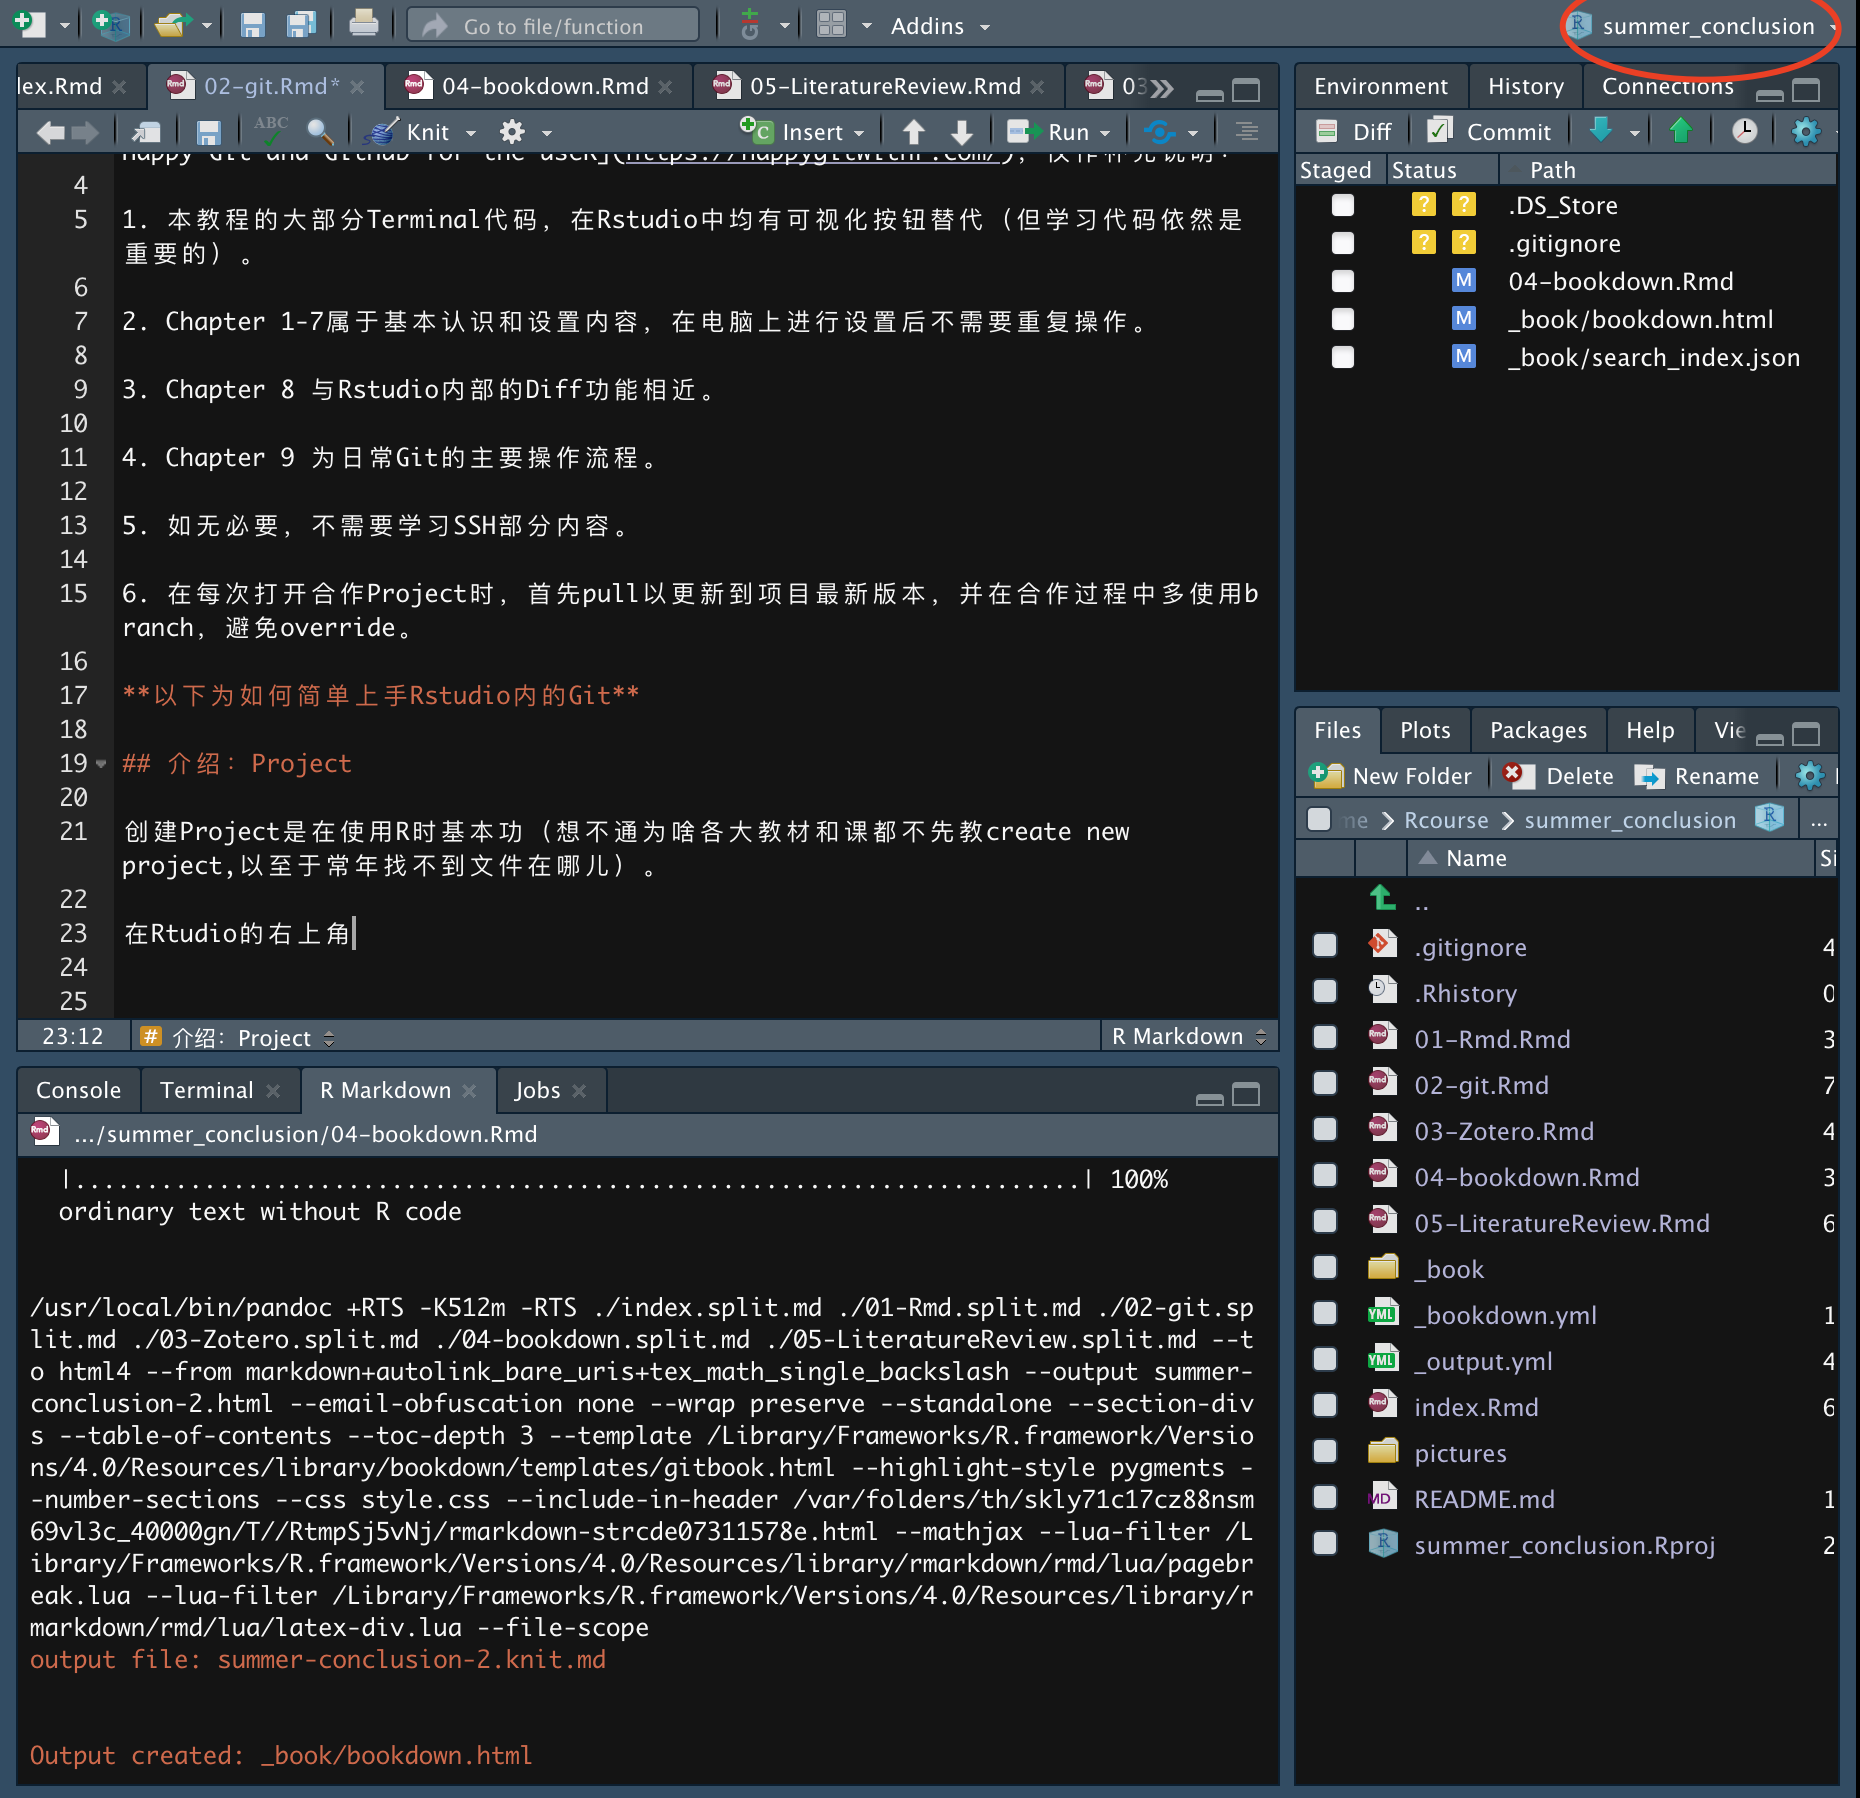
\includegraphics{./images/git_project.png}

\hypertarget{sec-clone}{%
\section{Clone已有repository}\label{sec-clone}}

对于公开或者有读取权限的repo,我们可以直接把它复制到本地,这个动作叫做克隆。
首先你要到对应远程平台上找到对应的\texttt{https}链接。

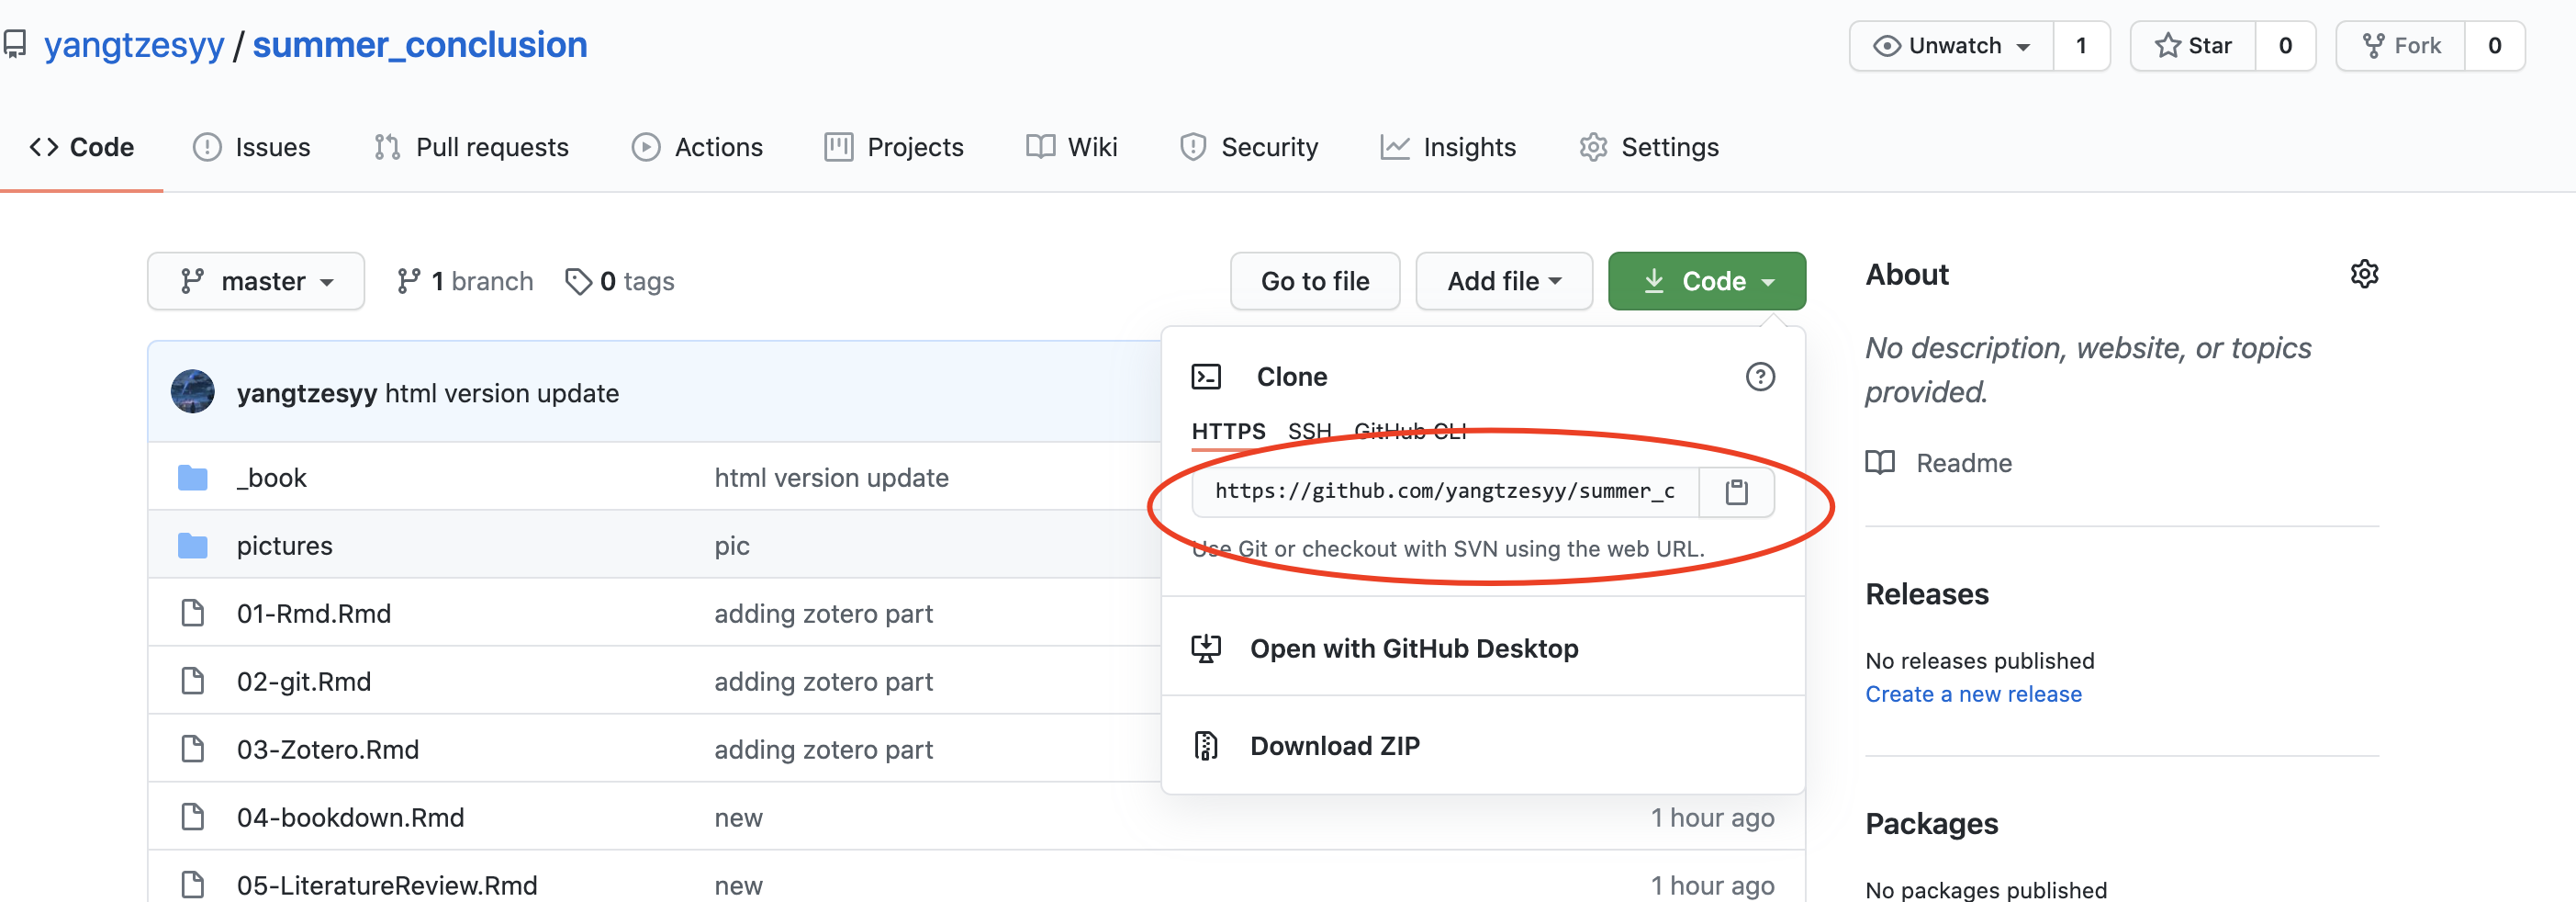
\includegraphics{./images/git_clone.png}

然后Rstudio中创建\texttt{New\ Project},选择\texttt{Version\ Control}→\texttt{Git}并复制https到对应窗口,选择文件夹位置,然后确定即可。

\hypertarget{ux521bux5efarepo}{%
\section{创建Repo}\label{ux521bux5efarepo}}

我们需要完成自己的Rstudio与Github账号的联动工作,才能写入Github上的repo。
但别担心,这只需要设置一次就能一劳永逸了。(\href{https://happygitwithr.com/credential-caching.html\#credential-caching}{英文教程})

首先,在github中创建一个token以表明身份,\href{https://docs.github.com/en/free-pro-team@latest/github/authenticating-to-github/creating-a-personal-access-token}{按照步骤}操作即可。Token类似于密码,需要小心保管。

现在,利用\texttt{credentials}包在R中储存Github账号信息。你需要将得到的Token输入到\texttt{set\_github\_pat()}中

\begin{Shaded}
\begin{Highlighting}[]
\FunctionTok{library}\NormalTok{(credentials)}

\FunctionTok{set\_github\_pat}\NormalTok{(Your Token Here)}
\end{Highlighting}
\end{Shaded}

你可以利用\texttt{gitcreds}包查看储存的Github账号信息。

\begin{Shaded}
\begin{Highlighting}[]
\FunctionTok{library}\NormalTok{(gitcreds)}

\FunctionTok{gitcreds\_set}\NormalTok{()}
\end{Highlighting}
\end{Shaded}

这时你可以直接到你使用的远程平台,找到创建库(New
repository)的按钮,按照步骤进行即可创建一个空的库。 然后你就可以利用
Section~\ref{sec-clone} 的方法将其克隆到本地。\footnote{其他两种建库的方式(将电脑中存在的project上传到Github中,将Github中已经存在的Project下载到电脑中)在\href{https://happygitwithr.com/new-github-first.html}{happygitwithr}有介绍。}

\hypertarget{addux548ccommit}{%
\section{Add和Commit}\label{addux548ccommit}}

首先在Rstudio里点击·Commit·

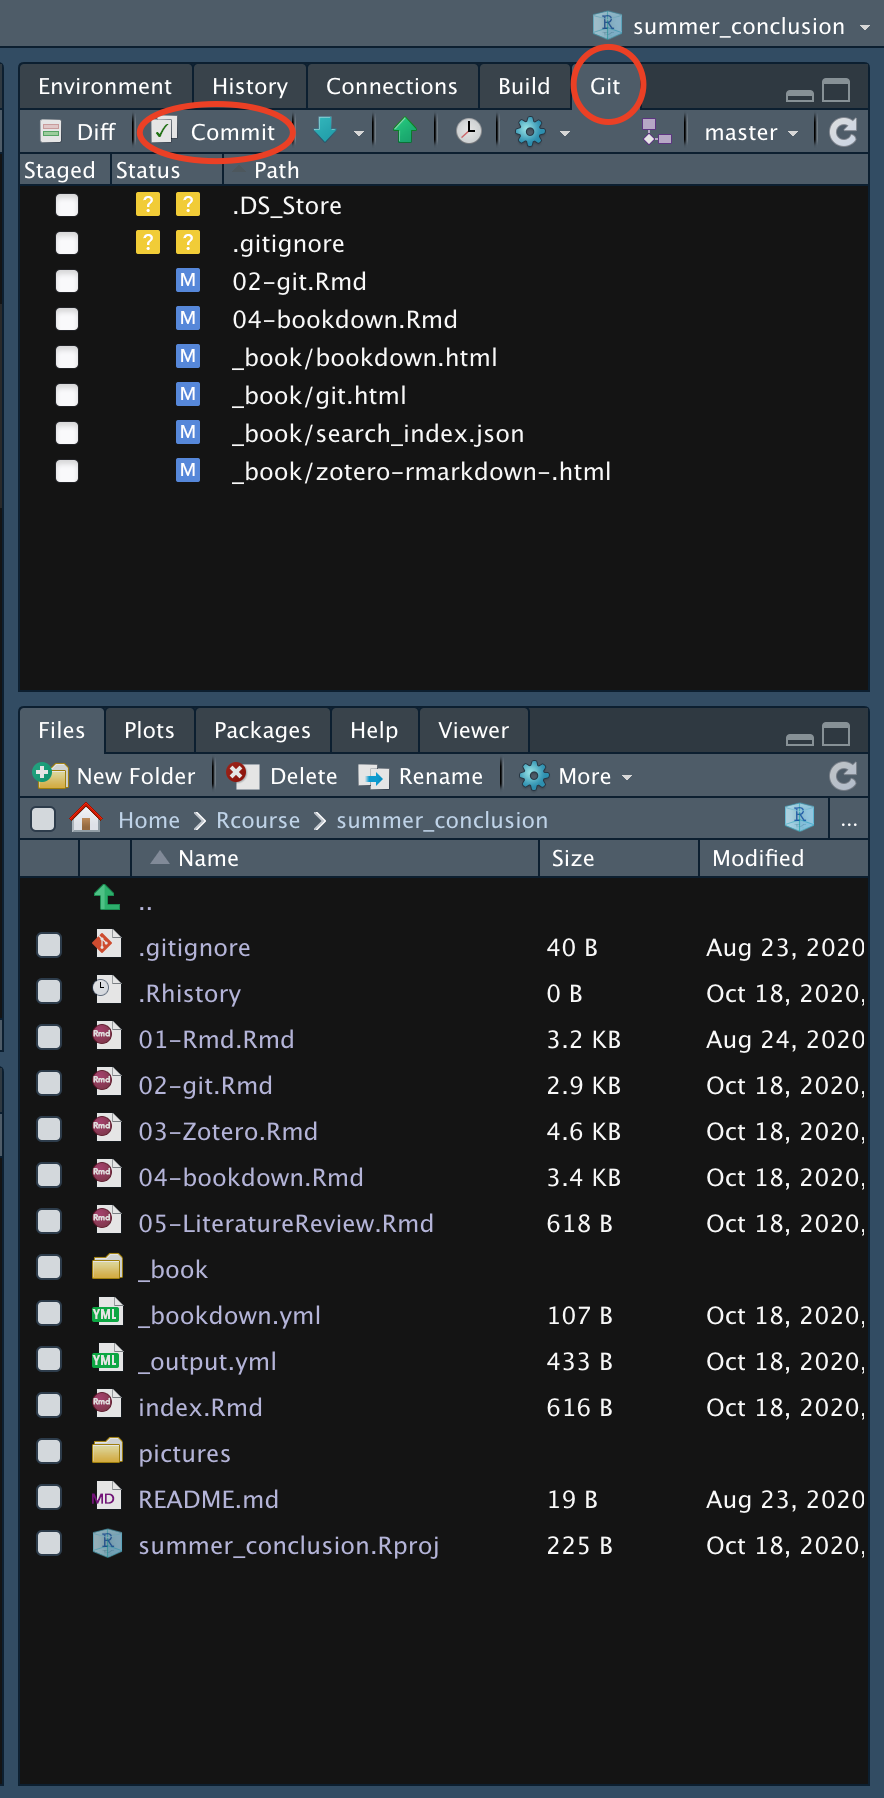
\includegraphics{./images/git_panel.png}

在Rstudio的\texttt{Git}部分有Commit栏,点进去,它会显示本地数据与云端数据(Github上)的区别(图片左栏)。左上显示有变化的文件,下方逐栏说明区别。

你可以使用stage确认变化(打勾)你可以面将想要进行版本控制的文件前面\texttt{Staged}里面进行勾选,或者使用以下命令(命令在Rstudio中的``Terminal''内输入):

\begin{Shaded}
\begin{Highlighting}[]
\NormalTok{git add \textless{}文件名\textgreater{}}
\end{Highlighting}
\end{Shaded}

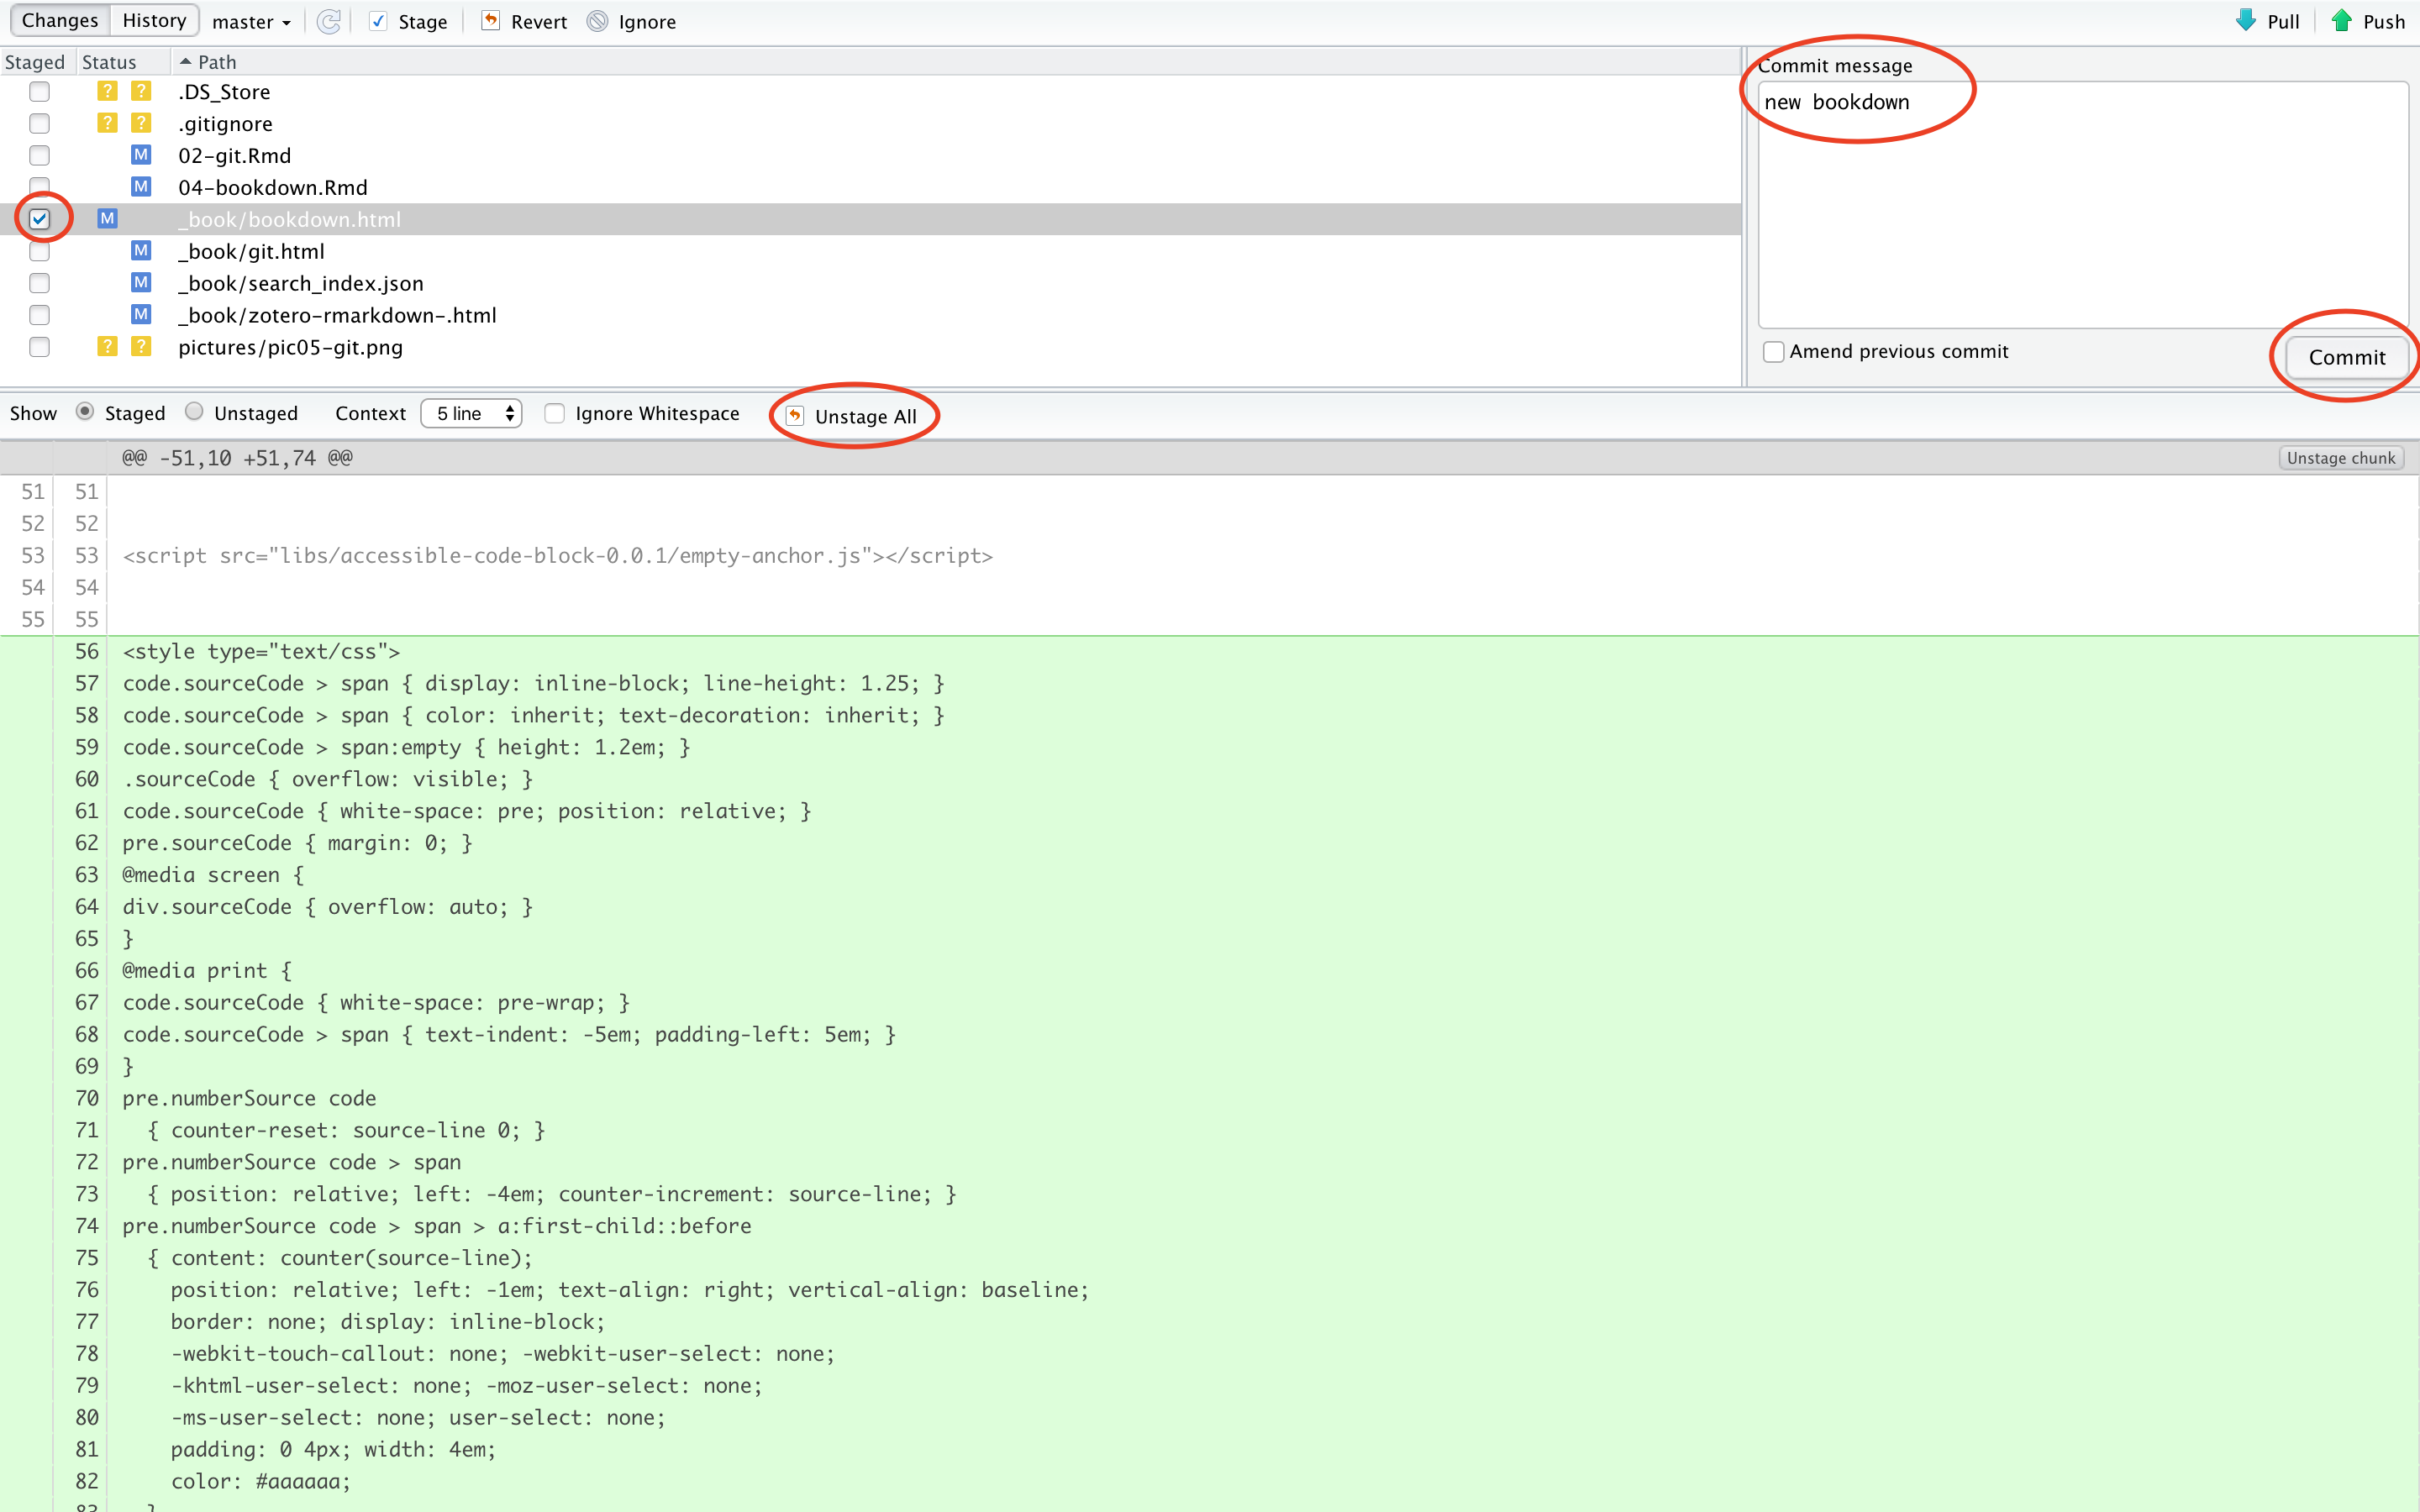
\includegraphics{./images/git_commit.png}

在确认完更改后,你需要输入commit信息,
通常是表明新版本特点的词、词组或一句话,并点击\texttt{commit}按钮确认。

这一步也可以通过以下代码完成:

\begin{Shaded}
\begin{Highlighting}[]
\NormalTok{git commit {-}m "\textless{}注释信息\textgreater{}"}
\end{Highlighting}
\end{Shaded}

\hypertarget{push}{%
\subsubsection{Push}\label{push}}

点击绿色向上箭头按钮,将本地更改上传到Github,或者直接输入命令\texttt{git\ push}。

\hypertarget{pullux517bux6210ux4e60ux60ef}{%
\subsection{Pull:养成习惯}\label{pullux517bux6210ux4e60ux60ef}}

再多人合作中,每次开始工作时,你需要先知道其他人对repo做了什么。一定要在每次工作前先将Github上的最新版本文件pull到本地中。

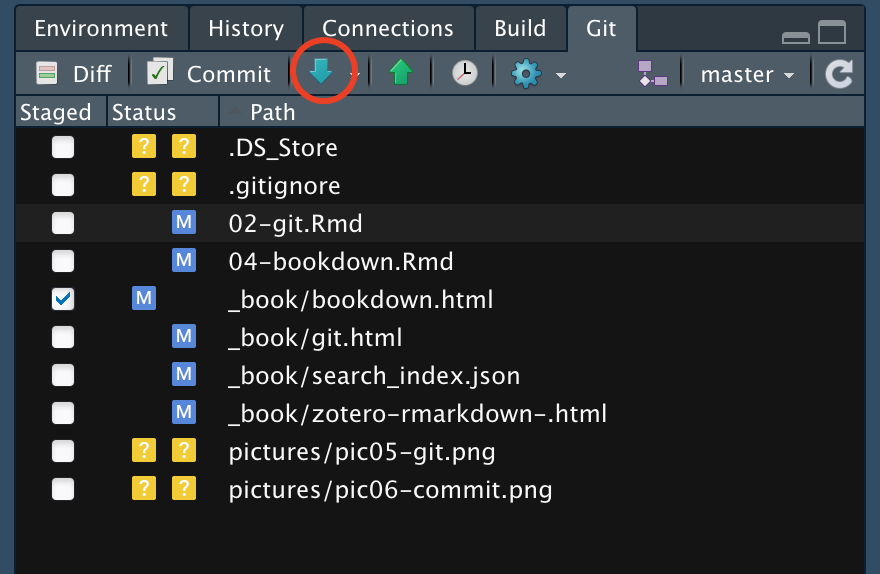
\includegraphics{./images/git_pull.png}

\hypertarget{branchux907fux514doverride}{%
\subsection{Branch:避免Override}\label{branchux907fux514doverride}}

你可以和朋友们各自创建自己的Branch(详细原理可见\href{https://happygitwithr.com/git-branches.html}{happygitwithr})。这相当于各自在不同的工作线上工作(因此不会将文件更改上传到master上)。我们仅需要将自己Branch中\textbf{完全确定}并\textbf{需要同他人共享}的部分上传到master上。

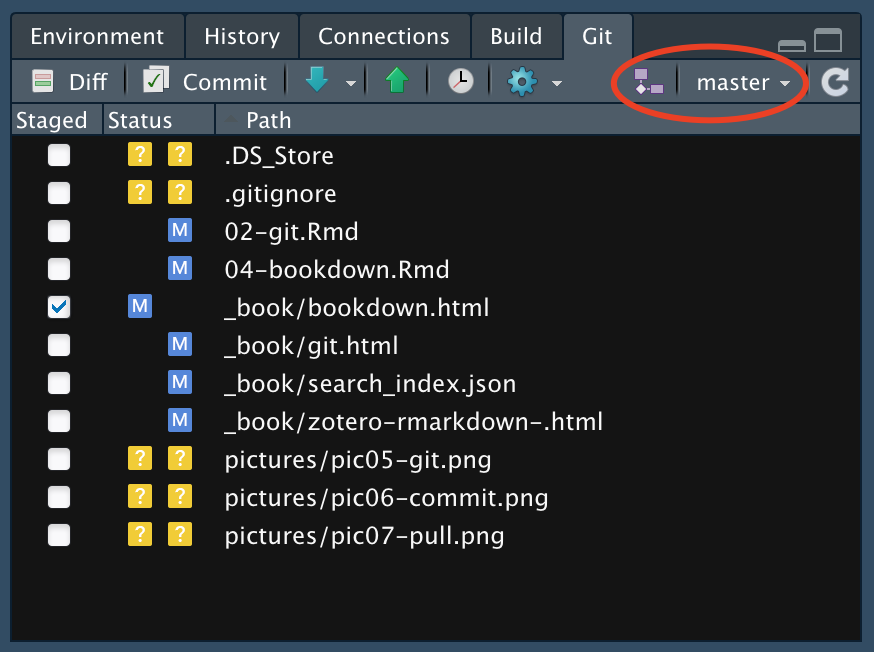
\includegraphics{./images/git_branch.png}



\end{document}
